%%
%% This is file `sample-acmsmall.tex',
%% generated with the docstrip utility.
%%
%% The original source files were:
%%
%% samples.dtx  (with options: `acmsmall')
%% 
%% IMPORTANT NOTICE:
%% 
%% For the copyright see the source file.
%% 
%% Any modified versions of this file must be renamed
%% with new filenames distinct from sample-acmsmall.tex.
%% 
%% For distribution of the original source see the terms
%% for copying and modification in the file samples.dtx.
%% 
%% This generated file may be distributed as long as the
%% original source files, as listed above, are part of the
%% same distribution. (The sources need not necessarily be
%% in the same archive or directory.)
%%
%% Commands for TeXCount
%TC:macro \cite [option:text,text]
%TC:macro \citep [option:text,text]
%TC:macro \citet [option:text,text]
%TC:envir table 0 1
%TC:envir table* 0 1
%TC:envir tabular [ignore] word
%TC:envir displaymath 0 word
%TC:envir math 0 word
%TC:envir comment 0 0
%%
%%
%% The first command in your LaTeX source must be the \documentclass command.
\documentclass[manuscript,screen,review,anonymous]{acmart}
\usepackage{emoji}
\usepackage{soul}
\usepackage{hyperref}
\usepackage{hyperxmp}
\usepackage[most]{tcolorbox}
\usepackage{lipsum}
\usepackage{xcolor}
\usepackage{multirow}
\usepackage{booktabs}
\usepackage{array}
\usepackage{rotating}
\usepackage{tabularx}
\usepackage{makecell}

\definecolor{linequote}{RGB}{224,215,188}
\definecolor{backquote}{RGB}{249,245,233}

\newtcolorbox{myquote}[1][]{%
    enhanced, breakable, 
    size=minimal,
    frame hidden, boxrule=0pt,
    sharp corners,
    colback=backquote,
    #1
}
% \documentclass[manuscript,review,anonymous]{acmart}
%% NOTE that a single column version is required for 
%% submission and peer review. This can be done by changing
%% the \doucmentclass[...]{acmart} in this template to 
%% \documentclass[manuscript,screen]{acmart}
%% 
%% To ensure 100% compatibility, please check the white list of
%% approved LaTeX packages to be used with the Master Article Template at
%% https://www.acm.org/publications/taps/whitelist-of-latex-packages 
%% before creating your document. The white list page provides 
%% information on how to submit additional LaTeX packages for 
%% review and adoption.
%% Fonts used in the template cannot be substituted; margin 
%% adjustments are not allowed.
%%
%% \BibTeX command to typeset BibTeX logo in the docs
\AtBeginDocument{%
  \providecommand\BibTeX{{%
    \normalfont B\kern-0.5em{\scshape i\kern-0.25em b}\kern-0.8em\TeX}}}

%% Rights management information.  This information is sent to you
%% when you complete the rights form.  These commands have SAMPLE
%% values in them; it is your responsibility as an author to replace
%% the commands and values with those provided to you when you
%% complete the rights form.
\setcopyright{acmcopyright}
\copyrightyear{2026}
\acmYear{2026}
\acmDOI{XXXXXXX.XXXXXXX}


%%
%% These commands are for a JOURNAL article.
\acmJournal{JACM}
\acmVolume{37}
\acmNumber{4}
\acmArticle{111}
\acmMonth{8}

%%
%% Submission ID.
%% Use this when submitting an article to a sponsored event. You'll
%% receive a unique submission ID from the organizers
%% of the event, and this ID should be used as the parameter to this command.
%%\acmSubmissionID{123-A56-BU3}

%%
%% For managing citations, it is recommended to use bibliography
%% files in BibTeX format.
%%
%% You can then either use BibTeX with the ACM-Reference-Format style,
%% or BibLaTeX with the acmnumeric or acmauthoryear sytles, that include
%% support for advanced citation of software artefact from the
%% biblatex-software package, also separately available on CTAN.
%%
%% Look at the sample-*-biblatex.tex files for templates showcasing
%% the biblatex styles.
%%

%%
%% The majority of ACM publications use numbered citations and
%% references.  The command \citestyle{authoryear} switches to the
%% "author year" style.
%%
%% If you are preparing content for an event
%% sponsored by ACM SIGGRAPH, you must use the "author year" style of
%% citations and references.
%% Uncommenting
%% the next command will enable that style.
%%\citestyle{acmauthoryear}

%%
%% end of the preamble, start of the body of the document source.
\begin{document}

\begin{teaserfigure}
    \centering
    \includegraphics[width=\linewidth]{images/Group 245 (1).png}
    \caption{(a) An ARG styled game, where participants are requested to upload labels of food products to discuss and analyze with the LLM; (b) a prompt suggesting the LLM to generate images when there is a shift in the game world; and (c) points and visualization of the point system through ASCII characters.}
    \label{fig:argPromptExample}
\end{teaserfigure}


%%
%% The "title" command has an optional parameter,
%% allowing the author to define a "short title" to be used in page headers.
\title{\textcolor{blue}{The TGP: The Taxonomy of Gamified Prompts, for Orchestrating Engaging Learning Experiences with Large Language Models}}



\renewcommand{\shortauthors}{Maram et al.}

%%
%% The abstract is a short summary of the work to be presented in the
%% article.
\begin{abstract}
\textcolor{blue}{The pedagogical use of Large Language Models (LLMs) often remains `transactional', prioritizing raw information transfer over learner agency and immersion. While Gameful Prompting, defined as the strategic embedding of game mechanics into system instructions, offers a scalable solution to this engagement gap, we currently lack a formal design language to bridge the gap between static prompting and dynamic play. In this paper, we address this by introducing the \textbf{Taxonomy of Gamified Prompts (TGP)}, a taxonomy for engineering prompts that embed systemic game mechanics, such as point economies, progression loops, and inventory management, directly into the LLM's operational logic. Through a participatory design process involving educators, students, and game researchers, we developed a corpus of 60 systemic gamified prompts for creating engaging learning experiences. Utilizing grounded theory analysis, we derive the TGP, the first comprehensive mapping of gamified prompt design, consisting of 5 primary dimensions and 19 sub-dimensions. We evaluate the taxonomy through a multi-stakeholder study, assessing its usability for prompt designers and measuring its impact on student immersion and emotional engagement. Our contributions provide a foundational toolkit for educators and designers to move beyond the chatbot paradigm and craft deeply engaging, mechanic rich, and adaptive game-based learning worlds.}
\end{abstract}

%%
%% The code below is generated by the tool at http://dl.acm.org/ccs.cfm.
%% Please copy and paste the code instead of the example below.
%%
\begin{CCSXML}
<ccs2012>
   <concept>
       <concept_id>10003120.10003121.10003124</concept_id>
       <concept_desc>Human-centered computing~Interaction paradigms</concept_desc>
       <concept_significance>500</concept_significance>
       </concept>
 </ccs2012>
\end{CCSXML}

\ccsdesc[500]{Human-centered computing~Interaction paradigms}
%%
%% Keywords. The author(s) should pick words that accurately describe
%% the work being presented. Separate the keywords with commas.
\keywords{Game Mechanics, Serious Games, LLMs, Taxonomy, Dataset}

\received{11 September 2025}
%\received[revised]{12 March 2009}
%\received[accepted]{5 June 2009}

%%
%% This command processes the author and affiliation, and title
%% information and builds the first part of the formatted document.
\maketitle


\section{Introduction} \label{introduction}

\textcolor{blue}{Large Language Models (LLMs) have rapidly transitioned from novel utilities to central infrastructure in education, assuming roles as varied as Socratic tutors, co-creative peers, and personalized illustrators \citep{hammer2024chatgpt, mollick2023using, maram2025listeninglanguagemodelsusing}. For the Human-Computer Interaction (HCI) community, these tools offer a compelling promise: the democratization of personalized scaffolding and learner agency \cite{adiguzel2023revolutionizing,chen2023artificial}. However, as adoption scales, a critical pedagogical tension has emerged. Recent studies warn of \textit{cognitive offloading}—a phenomenon where learners outsource mental effort to the AI, treating it as an `answer engine' rather than a thinking partner \citep{kosmyna2025your, fenu2024exploring}. The central challenge for the field is no longer providing access to AI, but designing interactions that resist passivity and sustain the ``productive struggle'' essential for deep learning.}

\textcolor{blue}{To address the integration of AI into classrooms, a new generation of orchestration platforms—such as Playlab.ai \footnote{\url{https://www.playlab.ai/}}, CircleIn \footnote{\url{https://www.circleinapp.com/}}, and Magic School AI \footnote{\url{https://www.circleinapp.com/}} have emerged. These tools have successfully lowered the technical barrier, allowing educators without programming skills to deploy custom AI assistants. Yet, while the \textit{access} problem is being solved, the \textit{design} problem remains: the resulting interactions are frequently transactional, linear, and inert \cite{gajos2022people, achiam2023gpt}. Without deliberate pedagogical structuring, these assistants often default to efficient information delivery, inadvertently encouraging the very passivity educators seek to avoid.}

\textcolor{blue}{We argue that embedding \textit{game mechanics} directly into LLM prompts offers a potent solution to this engagement gap. Game elements are not merely decorative; they function as cognitive forcing functions. By introducing constraints, role-play, uncertain outcomes, and resource management, we transform the LLM interaction from a static query-response loop into a dynamic system that demands planning and strategy. This approach leverages the ``magic circle'' of gameplay to create a safe space for experimentation, shifting the learner's role from a passive consumer of text to an active agent in a narrative.}

\textcolor{blue}{Historically, achieving this depth of cognitive engagement required \textit{Game-Based Learning (GBL)}—the development of standalone video games or complex simulations. While pedagogically effective, traditional GBL is hindered by specialized software development, substantial budgets, and extensive teacher training to implement. Furthermore, once built, these games are static artifacts, difficult for educators to customize for specific curriculum needs. We propose a scalable alternative: Gameful Prompting. We define gameful prompting as the \textit{strategic embedding of game mechanics—such as narrative roles, resource constraints, and rule-based feedback—directly into the system instructions of an LLM.} This approach transforms the general-purpose chatbot into a lightweight game engine. By orchestrating these mechanics through natural language, we capture the immersive benefits of GBL while retaining the accessibility and adaptability of standard AI tools, effectively democratizing the creation of educational games.}

\textcolor{blue}{Despite the promise of gameful prompting, a critical theoretical and practical gap remains. Established serious games frameworks, such as the Learning Mechanics–Game Mechanics (LM-GM) model \cite{arnab2015mapping}, were designed for deterministic software where rules are hard-coded. They offer little guidance on how to \textit{orchestrate} these mechanics in the probabilistic, unstructured environment of a Large Language Model. Educators are thus left with a powerful engine but no manual, raising the fundamental research question: \textbf{What game design elements and strategies can be embedded into LLM prompts to enhance student engagement?}}
\textcolor{blue}{This paper addresses this challenge by introducing the \textbf{Taxonomy of Gamified Prompts (TGP)}. Developed through a grounded theory analysis of collaborative design sessions with educators and students, the TGP bridges the gap between serious games theory and prompt engineering. It provides a structured vocabulary for designing prompts that function as a lightweight game engine. To validate this approach, our work makes the following contributions:}

\begin{enumerate} \item \textbf{A Corpus of Gameful Prompts:} We present a curated, open-access dataset of 60 gamified learning prompts. Co-designed with educators, this corpus serves as an empirical foundation, categorizing diverse strategies for transforming text-based interactions into playful, rigorous learning experiences.

\item \textbf{The Taxonomy of Gamified Prompts (TGP):} We introduce a novel design taxonomy that operationalizes abstract game mechanics into executable prompt patterns. The TGP provides educators and researchers with a conceptual toolkit to systematically design, analyze, and iterate on gameful LLM interactions.

\item \textbf{Evaluation of the Taxonomy:} We evaluate the TGP through a multi-stakeholder study. First, we assess the taxonomy's utility for prompt designers, measuring its impact on usability and cognitive load. Second, we evaluate the resulting prompts with students, measuring changes in immersion, attention, and emotional engagement compared to standard non-gamified baselines. \end{enumerate}
\section{Previous Work}

\subsection{LLMs in Education: Opportunities and Limitations}

\textcolor{blue}{Trained on vast text repositories, commercial LLMs support learning across diverse contexts by answering questions, generating content, and simulating dialogue \cite{achiam2023gpt,uppalapati2024comparative}. Research highlights their efficacy across various disciplines: in language learning, they reinforce grammar and fluency through adaptive conversation \cite{park2024align,koraishi2023teaching,ye2025position,zhang2024impact}; in computer science, they enhance computational thinking by assisting with debugging and explaining code logic \cite{ma2024teach,jin2024teach,tu2023should,molina2024leveraging}; and in the humanities, they support creativity and inquiry by simulating historical debates and co-creating design concepts \cite{guo2024prompting,vastakas2024cultural,chang2025framework,zha2024designing}. Additionally, LLMs offer immediate, personalized feedback that mirrors human quality \cite{dai2023can,jia2022automated}, enabling students to refine their work and reflect on their ideas in real-time \cite{tanwar2024opinebot,sessler2025towards}.}

\textcolor{blue}{Despite their potential, LLM-based chatbots present challenges in educational contexts. One concern is the challenge of sustaining engagement over time. Williams et al. \cite{williams2024ethical} and Fryer et al. \cite{fryer2020supporting} show that LLM chatbots initially capture students' interest due to their novelty, this enthusiasm often diminishes over time. Kooli et al. \cite{kooli2023chatbots} argue that students may become passive recipients of AI-generated responses, diminishing the active cognitive engagement necessary for deeper learning. As interactions become predictable or transactional, students may disengage, reducing the chatbot’s educational value.}

\textcolor{blue}{Kooli et al. \cite{kooli2023chatbots} point out that LLM chatbots have limited capacity to foster genuine emotional and social connections in learning environments. Effective education often relies on empathy, encouragement, and trust. While AI systems can simulate politeness or generate emotionally supportive responses, they lack true empathy and the nuanced understanding needed to form meaningful teacher-student relationships \cite{lin2024artificial}. Xiao et al. \cite{xiao2024review} reinforce this concern, noting that while chatbots can personalize content delivery and provide instant feedback, their emotional connection with students is inherently weaker than that of human educators.}

\textcolor{blue}{Beyond emotional limitations, there are notable pedagogical concerns associated with LLM-based chatbots. Huang et al. \cite{huang2022chatbots} argue that chatbots often produce generic responses that may fail to inspire creativity or critical thinking in learners. The uniformity of LLM generated responses can inadvertently promote surface-level learning. For instance, if students consistently receive similar AI-generated essay feedback, this homogeneity may reduce opportunities for students to develop unique writing styles or explore original ideas. Cenry et al. \cite{vcerny2023educational} observed that students often described conversations with chatbots as transactional and repetitive, resulting in reduced immersion and engagement. Similarly, Hellas et al. \cite{hellas2024experiences} and Lauricella et al. \cite{lauricella2023ludic} found that students reported chatbot interactions as monotonous and uninspiring, with AI responses often feeling mechanical and lacking depth. These findings suggest that the raw capabilities of the model are insufficient on their own; to prevent passivity and boredom, the interaction itself must be carefully structured and directed through intentional design.}


\subsection{Prompt Engineering for Education}
\textcolor{blue}{To mitigate the transactional nature of default LLM interactions, educators have turned to prompt engineering \cite{hedderich2024piece, wu2022ai, allen2023use}. Prompt engineering has emerged as a crucial skill for educators and learners using AI systems \cite{spasic2023using, cain2024prompting}. A prompt may range from a simple instruction, such as “Explain Newton’s laws in simple terms,” to more complex multi-part directives that outline step-by-step guidelines for the chatbot’s behavior \cite{pando2024prompting}. The structure, wording, and detail within these prompts significantly impact the quality and relevance of the AI’s responses \cite{walter2024embracing, mollick2024instructors}.}

Due to the critical role of prompt design, there is growing interest in exploring strategies for crafting effective prompts and training educators in these techniques \cite{park2024generative, eager2023prompting, wang2023unleashing}. One emerging strategy is prompt chaining, which involves breaking complex tasks into a series of smaller, sequential prompts. Each subtask’s output feeds into the next prompt, effectively creating a multi-turn pipeline to handle complex objectives. Sun et al. \cite{sun2024prompt} highlight how prompt chaining enables LLMs to handle sophisticated tasks, such as analyzing a student's essay and then generating customized quiz questions based on that analysis. Cain et al. \cite{cain2024prompting} emphasize the value of iterative prompt engineering, arguing that prompts refined through repeated testing and revision tend to produce more reliable and contextually appropriate responses. Iteration allows educators to refine their prompts by adjusting language, tone, or instructions to ensure better alignment with learning objectives.


Lan et al. \cite{lan2024teachers} highlight that the responsibility for crafting prompts often falls on instructors, many of whom lack formal training in AI-driven educational tools. This makes it challenging and time-consuming for instructors to design effective prompts. To address this, researchers have proposed structured frameworks that guide prompt creation. Lo et al. \cite{lo2023art} introduce a four-step framework designed to help educators create effective prompts. This framework emphasizes that prompts should (a) be precise, (b) provide clear context, (c) specify desired output formats, and (d) control the length and complexity of language. Such structured approaches empower educators to design prompts that yield coherent, informative, and contextually appropriate responses.

Similarly, Velasquez et al. \cite{velasquez2023prompt} present the Goal-Prompt-Evaluation-Iteration (GPEI) model. This framework follows four stages: (a) establishing the learning goal, (b) designing the prompt, (c) evaluating AI-generated responses, and (d) iterating on the prompt based on evaluation results. By following this structured process, instructors can refine their prompts to improve response accuracy, pedagogical alignment, and student engagement.

To further support educators, several online repositories and educational platforms now provide curated databases of effective prompts. Resources such as Learning Prompting\footnote{\url{https://learnprompting.org}}, ChatGPT Educational Resources\footnote{\url{https://openai.com/index/teaching-with-ai/}}, and specialized MOOCs on prompt engineering for educators\footnote{\url{https://www.coursera.org/specializations/prompt-engineering-for-educators}} offer practical guidance and sample prompts that instructors can adapt for their classrooms. Additionally, some LLM-powered tools, such as the Prompt Professor\footnote{\url{https://chatgpt.com/g/g-qfoOICq1l-prompt-professor}}, are designed to help educators construct effective prompts by suggesting improvements and refining prompt wording.

MacNeil et al. \cite{macneil2023prompt} argue that using predefined prompt templates can alleviate design, language, and time-related barriers that instructors face when developing prompts from scratch. Zamfirescu et al. \cite{zamfirescu2023johnny} highlight that prompt templates provide a structured starting point for instructors, especially when navigating unfamiliar pedagogical contexts. By offering adaptable templates, these resources empower instructors to construct effective prompts while addressing common challenges such as vague instructions, overly complex language, and time. Mollick et al. \cite{mollick2023assigning, mollick2023using} propose a taxonomy of LLM prompts in educational settings, prompts to mimic AI-tutors, AI-coaches, AI-mentors, AI-teammates, AI-tools, AI-simulators, and AI-students. Their taxonomy is supplemented by a curated prompt library that educators can use as a foundation for creating AI-driven learning experiences\footnote{\url{https://www.moreusefulthings.com/instructor-prompts}}. While this library does not critically analyze the design components of prompts, it serves as a valuable starting point for instructors seeking to experiment with prompt-driven educational strategies.

\textcolor{blue}{In addition to broad educational contexts, domain-specific frameworks are emerging to support instructors in specialized fields. Olla et al. \cite{olla2024ask} introduce a taxonomy of healthcare-related prompts designed to support medical educators in crafting context-specific LLM interactions. Similarly, institutions such as Harvard\footnote{\url{https://www.huit.harvard.edu/news/ai-prompts}} and UC Davis\footnote{\url{https://guides.library.ucdavis.edu/genai/prompt}} have developed educational resources that provide prompt templates tailored to specific academic disciplines. However, a critical gap remains in these existing prompt engineering frameworks. While they excel at ensuring clarity, accuracy, and functional utility (e.g., "explain X," "quiz me on Y"), they rarely address the motivational or immersive dynamics required to counter the student disengagement highlighted in the previous section. To move beyond transactional exchanges and foster deep engagement, we must look beyond functional instructions and explore how prompts can induce play and immersion.}



\subsection{LLMs for Game Based Learning}

\textcolor{blue}{An emerging solution to the engagement and emotional deficits of standard prompting is the integration of game elements into chatbot interactions. Historically, games for learning utilizing conversational agents faced limitations from fixed responses and restricted natural language capabilities \cite{gobl2021conversational,fadhil2017adaptive,othlinghaus2017supporting,jeuring2015communicate}. However, recent advancements in LLMs offer significant potential for developing dynamic, and playful educational chatbots \cite{bonetti2024using}. Huber \citep{huber2024leveraging} states that game-based learning via LLMs not only harness the creative affordances of LLMs but are also best positioned not as authoritative tutors but as gamemasters that co-construct rules, scenarios, and play.}

Stampfl \textit{et al.} demonstrate how students can engage in civic or professional dialogues with ChatGPT as a simulation partner \citep{stampfl2024role,stampfl2024revolutionising}. Their work highlights not only the increased immersion such systems offer but also the way the LLM’s improvisational capacity encourages deeper negotiation of meaning. Tódová \textit{et al.} \cite{todova2025quest} show how LLM-driven NPCs can sustain open-ended dialogue that maintain immersion and challenges students to think from multiple perspectives. Unlike traditional scripted NPCs, these characters embody misconceptions, ethical stances, or stakeholder perspectives that are central to inquiry-based learning, thereby expanding the epistemic role of NPCs from mere quest-givers to dialogic interlocutors.

In counselor education, Maurya \citep{maurya2024qualitative} show how ChatGPT can play the role of a client, allowing trainees to practice counseling strategies in low-stakes but realistic conversations. Breen \citep{breen2025large} experiments with historical simulations push this further, where LLMs generate branching character briefs that enable more nuanced explorations of past dilemmas. Kindenberg \textit{et al.} \cite{kindenberg2025role} building on role-playing note that LLMs reconfigure the design space for historical games by making adaptive scenario generation feasible within curricular constraints.

Beyond the use of LLMs as NPCs, Chen et al. \cite{chen2025characterizing} introduced an LLM platform that supports student learning through interactive storytelling. In addition to generating narratives, this chatbot provides visual content to enhance the storytelling experience. LLMs, with their extensive knowledge bases, have also simplified the creation of quiz games \cite{sreekanth2023quiz}. These quiz-games facilitate interactive narratives, allowing students to advance through levels or respond to progressively challenging questions while actively engaging with the chatbot \cite{sweetser2024large}.

Steenstra et al. \cite{steenstra2024engaging} presented a system that teaches adolescents about health education through an interactive narrative, where both the storyline and visual elements are generated by LLMs. Students are asked to select the right answer for questions generated by the LLM. Likewise, Caraco et al. \cite{caraco2025scaffolding} developed a chatbot-style game in which the LLM assigns programming and IT design tasks to help students enhance their system architecture skills. These studies collectively demonstrate promising results, illustrating how LLM-based chatbot games can support student learning via simulating real world scenarios. Zhang \textit{et al.} \cite{zhang2024simulating} take the logic of simulation further in their work on SimClass, a system where LLM-powered agents assume the roles of teachers and students to mirror classroom dynamics. Their studies show that multi-agent simulations help learners rehearse discourse strategies and anticipate peer responses, effectively creating a game of classroom participation. 

While educational applications of LLMs widely employ traditional tutoring, mentoring, and socratic methods, a significant gap remains in understanding precisely how instructors can leverage game elements and mechanics to impact learners. Our research addresses this gap by exploring game mechanics suitable for integration into LLM prompts and providing educators and instructional designers with a structured taxonomy for creating gamified prompts to support learning experiences. We acknowledge the benefits of gamified LLMs for learning that previous authors have demonstrated and extend existing work by proposing a comprehensive taxonomy that categorizes effective design elements to support the creation of gamified prompts. This taxonomy enables instructors and designers to develop playful, and pedagogically sound chatbot interactions while we examine both creator and learner perspectives. 

\textcolor{blue}{While these individual studies validate the potential of LLMs for game-based learning, they largely represent ad-hoc implementations. We currently lack a system for educators to construct these experiences. To systematically design these prompts, we must turn to established theories of serious game design and adapt them for the generative age.}



\begin{figure}
    \centering
    \includegraphics[width=\linewidth]{images/Group 96.png}
    \caption{Participant involvement across taxonomy development and evaluation phases. Activities span generative co-design, prompt collection, taxonomy construction, and evaluative studies measuring coverage, usability, and learning impact.}
    \label{fig:participant_involvement}
\end{figure}




\begin{figure}[!ht]
    \centering
    \includegraphics[width=\linewidth]{images/Group 247.png}
    \caption{(a) The architecture and API calls that support StudyHelper. (b) StudyHelper Playground: A platform to create prompts and test prompts. (c) StudyHelper Taxonomy Mode: A platform to explore the Gamified Prompts Taxonomy, create prompts and test prompts. (d) An illustration of how prompt creators can use the Gamified Prompt taxonomy while creating prompts.}
    \label{fig:StudyHelper}
\end{figure}



\subsection{Theoretical Frameworks for Serious Game Design} \label{theoretical_frameworks}

\textcolor{blue}{To transition from ad-hoc experiments to a structured design methodology, we must examine how gameplay and pedagogy have historically been mapped. Early work by Frasca \cite{frasca2013simulation} and subsequent classifications by Djaouti et al. \cite{djaouti2011origins} broke games down into ``Gameplay Bricks"—fundamental rules that define player manipulation and goals. While these atomic definitions (e.g., ``SHOOT", ``MOVE") allow for precise classification, they often operate at a low level of ``inter/action" that does not inherently carry pedagogical value \cite{arnab2015mapping}. As Marne et al. \cite{marne2012six} note, the principles of effective learning and engaging gameplay can be conflicting; mere interaction does not guarantee education.}

\textcolor{blue}{To bridge this gap, researchers developed frameworks focusing on context and immersion. Bellotti et al. \cite{bellotti2011designing} proposed ``sandbox" models where micro-games are embedded within larger 3D narratives, a structure proving effective in cultural heritage contexts. Similarly, Kenny and Gunter \cite{gunter2008taking} argued that learning content must be deeply immersed in the game's narrative rather than overlaid. These insights crystallized into evaluation-heavy frameworks like the Four-Dimensional Framework \cite{defreitas2006four} and the RETAIN model (Relevance, Embedding, Transfer, Adaptation, Immersion, Naturalisation). RETAIN correlates game design with learning theories like Keller’s ARCS \citep{li2018use}, ensuring game content promotes knowledge transfer. However, Westera et al. \cite{westera2019and} argue that these frameworks function primarily as evaluation guidelines—excellent for analyzing existing games but less prescriptive for the generative design of new ones.}

\textcolor{blue}{The most direct attempts to map structure to pedagogy come from Amory’s Game Object Model (GOM) \cite{amory2007game} and the LM-GM Framework \cite{arnab2015mapping}. GOM explicitly draws an analogy to Object-Oriented Programming (OOP), defining games as a set of interrelated ``objects" (e.g., Game Space, Actor Space) with abstract and concrete interfaces. While powerful for static software, this reliance on an ``object-oriented" metaphor reveals a critical limitation when applied to Large Language Models.}

\textcolor{blue}{Existing frameworks share a common assumption: the game engine is deterministic. In GOM or LM-GM, a designer ``selects" a mechanic (e.g., a resource bar) and ``implements" it via code. The relationship between the rule and the outcome is rigid. In contrast, LLM-based learning environments are probabilistic; the ``engine" is fluid text. We cannot simply ``instantiate" a Game Object in a chatbot; we must persuade the model to simulate one. This shifts the design challenge from implementation to orchestration. Our Gamified Prompts Taxonomy (G.P.T.) seeks to fill this void by operationalizing the high-level mappings of LM-GM and GOM into executable, natural-language design patterns.}



\section{Methodology}
In this section, we discuss the various steps taken to achieve our contributions, as illustrated in Figure~\ref{fig:participant_involvement}. First, we discuss a custom-built tool named StudyHelper that helps designers and instructors build, test, and iterate prompts. Next, we discuss: (a) developing a corpus of gamified prompts, (b) developing a taxonomy from the corpus of gamified prompts for learning, and (c) evaluating the taxonomy with regard to coverage, usability, and impact.


\subsection{Understanding StudyHelper}
StudyHelper comprises two complementary platforms: StudyHelper Playground (Figure~\ref{fig:StudyHelper} (b)) and StudyHelper Taxonomy Mode (Figure~\ref{fig:StudyHelper} (c)). Both modes support designers in iteratively refining chatbot prompts; in this case, to develop and iterate gamified prompts for learning (View Supplementary material for a video demonstration of StudyHelper).

\subsubsection{Prompt Creation in StudyHelper Playground} 
As shown in Figure~\ref{fig:StudyHelper} (a), StudyHelper leverages OpenAI's GPT-4o model as its core language processing engine, but distinguishes itself from conventional ChatGPT interactions through its systematic use of user-defined prompts to initiate the conversation and guide dialogue. For instance, consider Figure~\ref{fig:methodsIllustrations} (middle); here StudyHelper automatically initiates the conversation through an introductory message based on the underlying prompt. This architectural design ensures that all interactions remain precisely aligned with specific educational objectives and pedagogical goals. As illustrated in Figure~\ref{fig:StudyHelper} (b), there exists a panel where designers can enter their prompt instructions and click ``Create Custom GPT" to interact with their created prompt. All user-defined prompt iterations are automatically stored in a secure backend database, enabling creators to revisit and iterate upon their previous work over time. 

\subsubsection{Prompt Creation in StudyHelper Taxonomy Mode}
The StudyHelper Taxonomy Mode extends the StudyHelper Playground by enabling prompt creators to explore the proposed taxonomy. Prompt creators, educators, and researchers can access this comprehensive taxonomy by selecting ``View GPT Taxonomy" (Figure~\ref{fig:StudyHelper} (c)), which provides detailed access to various taxonomical dimensions, theoretical descriptions, and practical examples of constituent elements (Figure \ref{fig:StudyHelper} (d)). This taxonomy serves as both a reference guide and an inspiration source for prompt creators, helping them incorporate evidence-based gamification principles into their educational chatbot designs.

% \subsubsection{Learner Interaction:} From the learner perspective, they can access StudyHelper and interact with a curated library of prompts created by instructors and prompt designers. All student interactions with these prompts are logged and stored in the backend system for future analysis. 

% \subsubsection{Current Limitations of StudyHelper:} The implementation of StudyHelper used as part of the current study has certain limitations. First, the maximum allowed prompt length is 7000 words. This was deliberately chosen to optimize performance. Next, prompt creators were only allowed to use the GPT-4o model from OpenAI for this study. 



\begin{figure}
    \centering
    \includegraphics[width=\linewidth]{images/Group 239 (2).png}
    \caption{(left) Poster used to advertise Hackathon to use StudyHelper to create bots. (middle) Participants interacting and comparing various gamified prompts. (right) Instruction Slides given to participants to participate in class assignments}
    \label{fig:methodsIllustrations}
\end{figure}


\subsection{Contribution 1: Constructing a Corpus of Gamified Prompts for Learning}

Using the StudyHelper Playground, we organized three participatory activities to develop a corpus of prompts. The stakeholders for these activities were chosen to include a diverse group of creators with varying skill sets, such as human-centered design, game design, and pedagogy. The generative process consisted of (a) co-design sessions with instructors, (b) a hackathon among HCI and game design students, and (c) workshops among game design students. 

\subsubsection{Co-Design with Instructors} Through co-design sessions with three instructors, we developed four Gamified Prompts for Learning that instructors considered highly suitable for their classrooms. All three instructors were familiar with game-based learning, had previous research, teaching, and publication experience with regards to game-based learning, and self-reported to use AI regularly. After a demo of StudyHelper, instructors created gamified prompts to help students with their coursework. Instructors were free to iterate and test these prompts as part of the co-design sessions. In the co-design sessions, we included engineers to support any technical or AI-related queries, researchers from learning sciences to engage in discussions regarding pedagogy, and researchers associated with game mechanics to support discussions with regards to game mechanics. 

\subsubsection{Gamified Hackathon among Designers}
While instructor-led prompts are vital for understanding how LLMs integrate with pedagogy, students are also key stakeholders; understanding their vision for gamified learning is equally essential. To gather their perspectives and approach towards gamified LLM experiences for learning, we organized a gamified hackathon called ``Gamified Bot-a-thon,'' a competitive event hosted within the senior graduate students of the HCI and Game Design department at <A LARGE PUBLIC UNIVERSITY>. 

We aimed to leverage the expertise of senior graduate students in game design and HCI who have taken coursework with regards to AI, Human-Centered design, and game design. Participants actively used the Playground in StudyHelper to prototype, test, and refine their prompts. From this hackathon, we generated 16 prompts across a variety of topics like literature, finance, ethics, journalism, physics, and many more. To ensure appropriate motivation and high-quality prompts, the gamified hackathon had a net prize money of \$100.

\subsubsection{Gamified Learning Bot Creation Assignments}
To gain further prompts, we embedded the above hackathon as an  assignment into two game design courses at <A LARGE PUBLIC UNIVERSITY>. The students were senior game design students, with all participants claiming to have developed at least two digital games as part of their coursework. The first class consisted of 45 students and focused on AI, games, and the UX of AI. The second class consisted of six students and had a specific focus on developing games for change using AI. After discussion with the instructors to align with course objectives, the assignments were embedded into the curriculum to allow students to apply game and AI design principles. By directly involving students and, game designers in the generative process, we ensured the resulting prompts accurately reflected the elements that participants themselves found engaging and motivating. From this exercise, we collected 40 prompts. 


\subsection{Contribution 2: Building the Gamified Prompt Taxonomy}
\label{taxonomyBuilding}


\begin{figure}
    \centering
    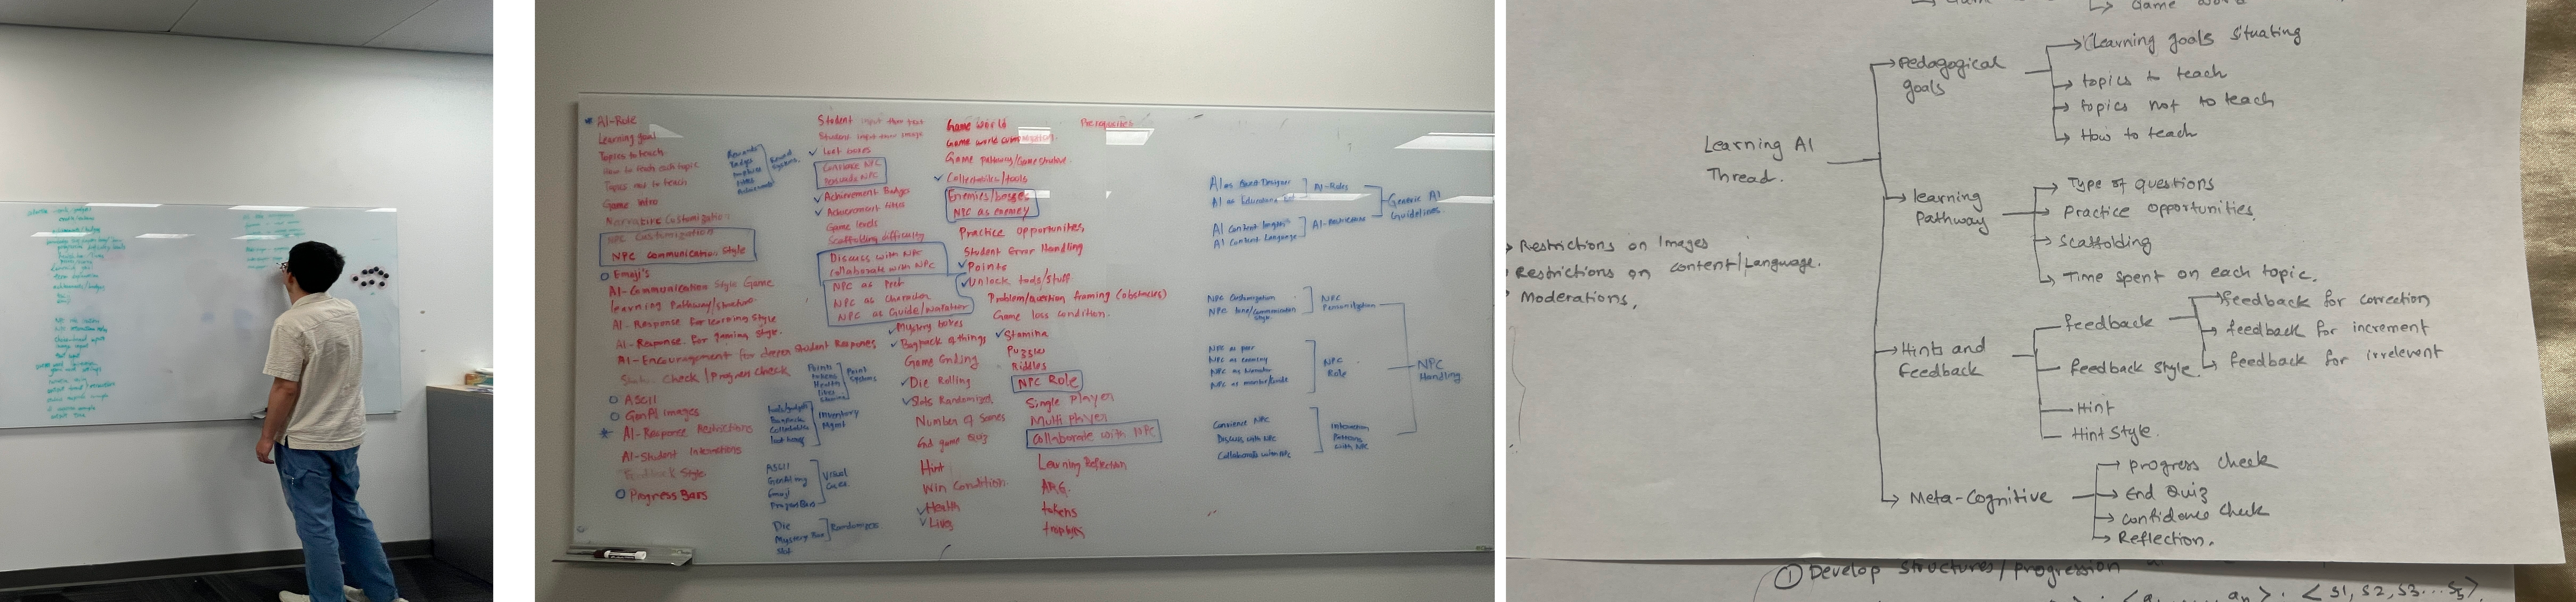
\includegraphics[width=\linewidth]{images/Group 199.png}
    \caption{Researchers developing the dimensions of the taxonomy through an iterative process}
    \label{fig:codebook-gen}
\end{figure}

The analysis of the 60 prompts generated from Contribution 1 began with two researchers applying a grounded theory approach inspired by Charmaz \cite{charmaz2006constructing,maram2022astraverse} to uncover key dimensions within the corpus of gamified prompts. All researchers involved in the process were experienced researchers in grounded theory, and published more then 1 research paper with regards to Games and AI. One researcher first segmented the prompts into fine-grained units. For this, the rationale we took is to answer the question to ``This part of the prompt asks the LLM to ....". Every time we identified a unit in the prompt that instructed LLMs to behave in a certain way, we marked it as a unit of analysis. The researchers then engaged in multiple collaborative sessions as illustrated in Figure~\ref{fig:codebook-gen}. The researchers used constant comparison to discuss refined the segments, identify emerging themes and gradually constructed a codebook encompassing 75 open codes, 19 axial codes, and 5 selective codes as illustrated in Figure~\ref{fig:GLPTax}. 

To establish reliability, both researchers independently coded 30\% of the dataset using the dimensions developed above. They calculated inter-rater reliability (IRR) with Cohen’s Kappa and iterated on each dimensions definition until they reached an IRR of 0.78, a threshold widely considered acceptable \cite{landis1977measurement,maram2024ah}. After achieving this level of agreement, the lead author independently coded the remainder of the dataset.


\begin{figure}
    \centering
    \includegraphics[width=\linewidth]{images/Screenshot 2025-08-29 115404.png}
    \caption{An illustration of Level 0, Level 1 and Level 2 prompts.}
    \label{fig:comparePromptLevels}
\end{figure}

\subsection{Contribution 3: Evaluating the Gamified Prompt Taxonomy}
\label{taxEval}

To assess our GPT taxonomy, we draw on established principles from taxonomy evaluation literature, particularly within information systems \citep{Nickerson2013method,Kaplan2022introducing,Pinto2024automatic} and HCI \citep{Tabassi2023aiuse,jeoung2025promptprism,maram2022astraverse,maram2023visual}. We operationalize this assessment through three constructs: \textbf{Coverage}, \textbf{Usability}, and \textbf{Impact}. These constructs are widely recognized as essential for evaluating knowledge organization systems. They ensure the taxonomy is comprehensive in scope and accurately represents the domain (Coverage) \citep{Pinto2024automatic, Mokkink2018cosmin, Nickerson2013method}, is practical, learnable, and efficient for its intended users (Usability) \citep{Pinto2024automatic, Tabassi2023aiuse, TaxonomyStrategiesUsability, Das2017human}, and is demonstrably beneficial in improving the quality of outcomes derived from its use (Impact) \citep{Bowman1999interaction}. In the subsequent paragraphs, we discuss how we evaluate the taxonomy with regards to coverage, usability and impact. 


\begin{figure}
    \centering
    \includegraphics[width=\linewidth]{images/Group 229 (1).png}
    \caption{The GPT illustrated with examples, and all the levels of codes.}
    \label{fig:GLPTax}
\end{figure}


%\begin{itemize}
%\item 
\textbf{Coverage:} We evaluated coverage to verify that any gamified prompt for learning, regardless of its complexity or specific gamified nature, can be appropriately situated and classified within the taxonomy's structure \citep{Pinto2024automatic, Nickerson2013method, Kaplan2022introducing}. To assess coverage, we conducted a Game Design-AI workshop where we invited game designers to construct gamified prompts for learning without prior exposure to our taxonomy. Since we intend the taxonomy as a design support tool rather than a fixed curricular framework, testing it with participants skilled in design thinking and creativity provides meaningful insights into its coverage and robustness \cite{sanders2008co,deterding2011game}.

Each participant reported building a portfolio of at least three games previously, including at least one game for learning purposes. This background equipped them with the ability to creatively generate prompts, identify mechanics, and test the taxonomy's adaptability across diverse scenarios. 

The workshop generated a total of 21 distinct prompts. Similar to the taxonomy building step, researchers broke down each prompt into granular elements and identified how the prompts fall within the design space of the taxonomy (or not). 

%\item 
\textbf{Usability (Ease of Creation and Guidance)}: We wanted to ensure that the taxonomy is an efficient and helpful tool for creating gamified prompts for learning \citep{jeoung2025promptprism, TaxonomyStrategiesUsability}. To evaluate this, we invited 34 stakeholders. The stakeholders consisted of five active instructors, seven teaching assistants (who were also researchers), and 22 junior game designers who self-reported having built at least two functional games in the past and having experience with AI and Games. This study employed a within-subjects design, where each participant created gamified prompts for learning under two randomized conditions: once without the taxonomy and once with its aid. Participants independently developed a gamified LLM prompt using the StudyHelper's playground (see Figure~\ref{fig:StudyHelper} (b)) and then completed a task utilizing the proposed taxonomy through the StudyHelper’s ``Taxonomy Mode," which was designed to help designers systematically explore and apply gamified elements (see Figure~\ref{fig:StudyHelper} (c) and (d)) \citep{TaxonomyStrategiesUsability, jeoung2025promptprism}.

Following these tasks, stakeholders completed the NASA-TLX (Task Load Index) \citep{hart1988development} and TAM (Technology Acceptance Model) \citep{davis1989technology} surveys. These instruments were specifically chosen to provide a comprehensive picture of usability. The NASA-TLX allowed us to measure the perceived workload of the creative task itself, assessing dimensions like mental demand, effort, and frustration in creating gamified prompts. This was crucial for quantifying whether the taxonomy made the process less cognitively demanding. In parallel, the TAM survey evaluated the designers perception of the taxonomy as a tool, focusing on its Perceived Usefulness (Does it help me create better prompts?) and Perceived Ease of Use (Is the taxonomy itself easy to apply?). 

%\item 
\textbf{Impact}: To measure the impact of our proposed taxonomy, we evaluated it from the perspectives of two stakeholders: prompt creators and end-users. From prompt creators, we gathered qualitative insights as part of the usability test described above, where participants answered optional open-ended questions about their experience. 

From the students' perspective, we hypothesized that an effective taxonomy should enable instructors to design prompts that students find more engaging and immersive. To test this, we conducted an experiment with 10 students recruited from <A LARGE PUBLIC UNIVERSITY>, who interacted with prompts on two topics: climate change and basic math. For each topic, participants were presented with three distinct prompts representing varying levels of design sophistication. The first was a control prompt developed by a pedagogy researcher—a standard instructional prompt without gamified elements. The second was a prompt developed by an instructor without using our taxonomy, while the third was a prompt created by another instructor who utilized our taxonomy. Throughout the paper, we refer to these three prompts as Level 0 (L0), Level 1 (L1), and Level 2 (L2) prompts. An illustration highlighting the differences between the three levels of prompts is presented in Figure~\ref{fig:comparePromptLevels}. Given the sample size of 10 participants, we employed a mixed-methods approach. Participants completed a semi-structured interview discussing their experiences with each prompt. To complement their qualitative insights, participants provided quantitative data from specific subscales of three validated instruments. To assess immersion and engagement, we used the designated immersion and engagement questions from the Player Experience of Need Satisfaction (PENS) \cite{ryan2006motivational}. We measured enjoyment, a core component of intrinsic motivation, using the Interest/Enjoyment subscale of the Intrinsic Motivation Inventory (IMI) \cite{ryan1983relation}. Finally, to gauge cognitive absorption and focus, we used the Attention Quality subscale from the Situational Interest Survey \cite{linnenbrink2010measuring}. The selection of these specific subscales allowed us to measure key indicators of a engaging and immersive user experience.  
%\end{itemize}



\section{Results}
In this section, we first present the prompt corpus (Contribution 1), followed by the taxonomy (Contribution 2) and, subsequently, the evaluation of the taxonomy (Contribution 3)

\begin{figure}
    \centering
    \includegraphics[width=\linewidth]{images/Group 241.png}
    \caption{(left) Number of gamified prompts made across various learning topics. (right) Density of taxonomy elements distributed across the corpus of gamified prompts.}
    \label{fig:distributions}
\end{figure}



\subsection{Contribution 1: The Gamified Prompts for Learning Corpus}
\label{c1}

Through our various prompt generation activities, we obtained a total of 60 prompts. To the best of our knowledge, this is the first available corpus of prompts focused on gamified learning interactions with LLMs. For the larger community benefit, we share all the corpus in the format illustrated in Figure \ref{fig:corpusPromptExample} -\footnote{URL redacted for review} and in our supplemental materials.

As illustrated in Figure \ref{fig:distributions}, the prompts were distributed across topics such as programming, STEM (math, physics, chemistry, statistics, probability), life skills (cooking, healthcare, farming, banking), research and ethics (research methods, ethical research), climate and environment (climate change, ocean cleanup), humanities (literature, history, art), and other various topics. This reflects the diversity of the corpus, and the wide range of topics that can adapt a gamified approach for learning via LLMs. 

The average length of a prompt was 394 words, with 43 prompts being under 500 words, 10 prompts between 500-750 words, two prompts between 751-1000 words, and, finally, five prompts between 1001-1500 words. As mentioned in Section \ref{taxonomyBuilding} we identified  identified 960 units to analyze across the 60 prompts. As illustrated in Figure \ref{fig:corpusPromptExample}, for each prompt we tag it with the appropriate mechanics and elements found allowing users to query across the corpus. In the subsequent section, we analyze the 960 prompts to establish the Gamified Prompt Taxonomy for designing engaging learning experiences via LLMs. 

\begin{figure}
    \centering
    \includegraphics[width=\linewidth]{images/Group 243 (1).png}
    \caption{A prompt from the prompts corpus with appropriate codes highlighted. As illustrated, the corpus website [URL Redacted for review], will allow users to search, query prompts based on tags, and will allow users to interact with the prompts. Further, the prompt shown results in the interactions demonstrated.}
    \label{fig:corpusPromptExample}
\end{figure}


\begin{figure}
    \centering
    \includegraphics[width=\linewidth]{images/Group 244 (2).png}
    \caption{(a) A multiplayer gamified learning prompt collecting user name (names changed for anonymity) and role; (b) A prompt teaching programming, using titles and achievements to motivate players; and (c) A DnD styled gamified learning prompt, uses randomization in the form of die rolls within the gameplay.}
    \label{fig:multiPlayerPromptExample}
\end{figure}
 


\subsection{Contribution 2: Core Taxonomy Structure }
\label{c2}

As illustrated in Figure~\ref{fig:GLPTax}, the taxonomy encompasses five selective codes: \textbf{Game Mechanics}, \textbf{AI Control}, \textbf{The Teacher}, \textbf{Game Director}, and \textbf{NPCs}. Each selective code contains multiple axial codes that further decompose into specific open codes, creating a hierarchical structure. In this section, we discuss each selective code and the underlying axial and open codes. 

\subsubsection{The Game Director}

The \textbf{Game Director} selective code encompasses the structural elements that define how gamified learning experiences unfold over time. The \textbf{Game Type} axial code reveals diverse approaches to player interaction, ranging from regular single-player games to more complex multiplayer and ARG framings. While within the corpus, most prompts are regular single player games, we noticed that some prompts encouraged more than one player to interact with the chatbot at once. In this situation, the AI serves as the moderator, dictating the turns and tasks for each player. For example, in a prompt aiming to teach ethical journalism, a multiplayer element is includes as follows in the prompt - \textit{``First ask all the names of the players and assign them roles. Assign roles to each player like the Boss, Journalist, Social Media Influencers. For each turn, give [....]"}. An interaction for this prompt is illustrated in Figure~\ref{fig:multiPlayerPromptExample} (a). Given the ability to comprehend images, we noticed a few prompts encouraging players to submit images to progress in the game. For instance, a programming-based game stated - \textit{``Have users submit, hand written code and provide feedback after analyzing the hand written code".} On a similar tangent as illustrated in Figure~\ref{fig:argPromptExample} (a), a prompt aiming to teach sugars and ingredients mentioned - \textit{``In this challenge, give specific tasks, prompting students to upload food label images [....]".} 

The \textbf{Game Conditions} axial code is responsible for establishing clear win and loss states, introductions and closure to the game. The establishment of winning and losing states is crucial to inform the players of their gaming goals, and to determine when to stop the game. A prompt teaching statistics defines success in their prompt - \textit{``mastery demonstrations of statistical concepts needed for exam preparation and finishes all the interactions with NPCs.''} - while a prompt teaching survival-skills through a forest narrative creates explicit failure conditions where \textit{``The moment the creature catches up with the player, they loose.''}. 

The \textbf{Game Pathway} axial code structures the temporal flow of learning experiences through carefully designed introductions, level progressions, and culminating activities. A bot teaching climate change exemplifies pathway design with its elaborate introduction - \textit{``You have been chosen to join the Guardians of Earth, a secret league dedicated to protecting our planet, in the first level [....], in the next habitat [....]''} followed by progressive challenges that increase in complexity. Essentially, the Game Pathway provides structure in terms of how to start the game, how to progress the game, and, finally, how to end the interaction in the game. 

The \textbf{Game World} elements create immersive contexts that situate learning within compelling fictional environments. For instance, a bot aiming to teach probability and finance situates players in Las Vegas as a Casino host - \textit{``You are to act as a Casino host for a roulette game in the MGM at Las Vegas, taking in all the possibilities for a single 0 roulette game [...]"}. Similarly, another prompt aiming to teach players about Python programming illustrates this by placing the player in space - \textit{``The theme of this lesson is `Stranded In Space' where the player is trapped inside of a spaceship. They will need to get the spaceship into working shape and navigate it back to Earth."} Similarly, as illustrated in Figure~\ref{fig:corpusPromptExample}, the player is allowed to choose their own world, and the LLM crafts the NPCs and narratives according to the selected game world. 

\subsubsection{Game Mechanics}
The \textbf{Gameplay Mechanics} selective code represents the most recognizable aspects of gamification, encompassing the reward systems and mechanics that transform educational interactions into game-like experiences. The \textbf{Reward/Points System} axial code emerges as a central motivational structure, manifested through achievements, badges, trophies, titles, and point systems that provide immediate feedback and recognition for learning progress. Previous scores/points are stored in the conversation, and when a player takes an action in chat, a corresponding manipulation is done to the points. For instance, a prompt aiming to teach literature has \textit{``a weighted point system, where players are awarded more points for deeper analysis of the character, rather then [sic] surface level observations"}. Similarly, as illustrated in Figure~\ref{fig:multiPlayerPromptExample} (b), as users finish various tasks, they are awarded points, which also result in them receiving specific badges. 

Apart from the use of points, we noticed the use of Titles, Trophies, Badges, and Medals to provide immediate feedback, and gratification for students. For instance, in a prompt aiming to teach climate change, we saw the prompt - \textit{``Provide the sage, a Bronze Medal \emoji{3rd-place-medal} for basic environmental awareness, Silver Medals \emoji{2nd-place-medal} for implementing conservation strategies, and Gold medals \emoji{1st-place-medal} for designing comprehensive sustainability solutions."} This tiered medal system creates clear progression pathways while recognizing different levels of mastery within the same conceptual domain. 


The \textbf{Survival System} introduces risk and consequence elements through \textbf{health}, \textbf{lives}, and \textbf{stamina} mechanics that add urgency and strategic thinking to educational interactions. A prompt aiming to teach probability situated in a haunted house demonstrates this approach by stating  \textit{``The player gets 3 lives, and they can progress through rooms as long as they can"}. Similarly, a prompt teaching math employs health points, where they include the following - \textit{``navigate the dungeon, where each problem answered wrong reduces health points, the adventurer can recover health points when they meet Dr.Pythogres"}.


\textbf{Inventory Management} systems create engagement through collectible items, tools, and resources that students accumulate and use throughout their learning journey. The conversation stores items and tools the players have been given or gathered as part of their progression. For example, a prompt teaching sugar and food ingredients states - \textit{``Allow the players to pull any of the detective tool to find hidden sugars in the image"}. Further, a climate change prompt mentions - \textit{``Form the climate armory, allow users to choose the \emoji{water-pistol} Plasma Shooter, \emoji{sponge} Pollution Sponge, to tackle the climate catastrophe"}. Similarly, as illustrated in Figure~\ref{fig:multiPlayerPromptExample} (c), the user is provided options to add an item into their inventory. 


The last approach was the use of \textbf{Randomization}. For instance, as illustrated in Figure~\ref{fig:multiPlayerPromptExample} (c), we notice how the player is provided with a die whose outcomes determine the fate of the player as they navigate a dungeon. Similarly, we saw other randomization such as loot boxes, slot machines, and mystery boxes to add an element of surprise and have the gameplay adjust based on the items received in the boxes. For instance, in a prompt teaching finances provided opportunities to gamble money in slot machines to illustrate how it could be a bad practice - \textit{``players are allowed to spend money on a slot machines [sic], allow them insert their money in multiples of 10".} Similarly, 

\subsubsection{The Teacher}

The \textbf{Teacher} selective code contains the educational elements that make these prompts effective learning tools. This is where game mechanics meet actual teaching and learning goals.

The axial code \textbf{Pedagogical Goals} defines what students should learn and how they should learn it. The pedagogical goal part of the prompt instructs the LLM on \textbf{Topics to teach}, \textbf{Topics not to teach}, and information on \textbf{How to teach the topic}. For example, in the corpus one prompt states - \textit{``Your goal it [sic] to teach students foundations of Mathematics."}. Next, a prompt teaching climate change explicitly mentions to focus on certain topics while avoiding other topics - \textit{``Make sure the discussion revolves around scientific facts on causes of climate change and not political debates about climate change".} This ensures the LLM is situated to teach only topics the instructors want the students to learn. Similarly, as illustrated in Figure~\ref{fig:corpusPromptExample}, the instructor, apart from mentioning what topics to teach (t-tests, ANOVA), advises the LLM to stay away from topics such as two-way ANOVA and Chi-square. By instructing the LLM on what topics to teach and not to teach, the learning is aligned with the goals of the class or instructor. 

The \textbf{Learning Pathways} axial code captures how to sequence learning material within the game. For instance, a prompt aiming to teach players permutations and combinations through Blackjack stated - \textit{``First explain the different cards in a playing deck, and the number of cards, [...], explain the definitions of permutations and combinations, use the cards to show the examples. Encourage players to explain their thinking."} Here, we notice the step-by-step approach to provide granular information instead of feeling overwhelmed by difficult concepts too early. Another prompt, aiming to teach programming for children, mentions - \textit{``I want at least 3 interactions for each level. Before the interaction takes place, have the NPC provide some information on the topic of the level so the student can be given information about the topic before being presented a challenge. Please do not print out the entire level into one response. If the player gets stuck allow the student to ask the NPC for the level to help them out. Do not directly tell the student how to clear the encounter until they have asked for help at least 3 times."} The prompt clearly lays out the structure in terms of how they want the students to interact with the bot and how the LLM should present its learning goals. Such a structured approach is also evident in Figure~\ref{fig:multiPlayerPromptExample} (b), where the prompt first introduces the concept of variables, and then moves onto arithmetic operations. 

\textbf{Hints and Feedback} systems help students when they are stuck in a particular task, or provide corrective measures when students get answers to questions wrong. For instance, in a prompt aiming to teach students research methods, the prompt guides students to think about the correct approach instead of having the prompt directly provide answers to questions they answer wrong - \textit{``When students give a response, ask them to explain their reasoning before going to the next question, however if they get an answer wrong, instead of giving the answer, provide hints that help them think critically and reach the answer."}

The \textbf{Metacognitive} elements help students think about their own learning. In the corpus, a bot aiming to teach research methods regularly checks in with students about how confident they feel about different research concepts, and if they are ready to move on to the next segment - \textit{``After reach section, ask students how confident they feel in the section, ask them to rate their confidence between 1-5. If they share a low confidence score, gather information with that the student is not confident about and provide more examples on the topic."} This is also evident in Figure~\ref{fig:corpusPromptExample}, where players are requested to rate their confidence before moving on to the next confidence. Other approaches use reflection, including asking players to summarize their experience and reflect on their experience. For instance, a prompt for a bot aiming to teach Aztec history, includes - \textit{``After the last level, ask players to reflect on the various NPCs and summarize their conversations and strategies used to expand their empire". }


\subsubsection{AI Control}

The \textbf{AI Control} selective code addresses the technical and procedural aspects of AI behavior that ensure consistent, appropriate, and effective interactions. The \textbf{Output Control} axial code involve instances in the prompt that guide the output of the AI responses. For instance, across iterations, we noticed participants found the AI responses to be long and verbose, and to counter this, designers often included - \textit{``Keep your response between 200 to 400 characters"}. To illustrate this difference, consider Figure~\ref{fig:multiPlayerPromptExample} (a) and (b). The first prompt requests the LLM to keep the response limited to 150-300 characters, resulting in shorter LLM responses, while the second prompt does not mention any such restriction, resulting in the LLM providing longer responses. Further, we noticed that designers placed language restrictions and and output moderation to  ensure that the generated text and images generated are educational and do not digress from the main topic.

The \textbf{Input Control} axial reveals approaches to how players interact with AI systems. Apart from images and regular text-based input, other input mechanics included  \textbf{Choice-based input systems} where students are provided with a set of options which they are free to choose from. For example, a prompt aiming to teach about sustainable fishing practices mentions - \textit{``Let users choose among the following options for their fishing camp \emoji{keycap-1} Lake Fork, \emoji{keycap-2}, [....]"}. This is also evident in Figure~\ref{fig:argPromptExample} (b), where users are provided an option to choose which aspect of the game world they want to explore.

Apart from text, LLMs have taken strides in generating images. Given this advantage to make the game experience more playful, designers took advantage by incorporating \textbf{Visual elements} in AI responses. Visual elements provide immediate aesthetic feedback through multiple modalities that transform text-based interactions into rich sensory experiences. In a prompt titled the Physics Dungeon, the player uses \textit{ASCII} as a form of art to create mazes - \textit{``Create 10×10 matrix visual representations using ASCII characters to show the dungeon layout, player position, and discovered pathways.''}. An illustration of this is also evident in Figure~\ref{fig:argPromptExample} (c), where the task of the player is to climb a tower and the tower is demonstrated using ASCII. Similarly, we notice in Figure~\ref{fig:argPromptExample} (b) how various scenes as described in the prompt are illustrated to the players to situate players within the game world.

\textbf{Emojis} serve dual functions as both aesthetic enhancement and information encoding systems. A prompt titled Climate Quest employs emojis - \textit{``\emoji{earth-africa} Climate Quest,'' ``Welcome, Explorer! \emoji{earth-americas}\emoji{sparkles}''}  as consistent symbolic representations of different environmental concepts. Apart from helping to frame the game world, emojis help in providing clarity on other design elements. For instance, survival mechanics such as hearts, powers, and collectibles were  represented by emojis. A prompt teaching physics instructed -  \textit{``Always place the Health Bar (10 hearts) at the start of the message and the Progress Bar at the end... Health: \emoji{heart}\emoji{heart}\emoji{heart}\emoji{heart}\emoji{heart}\emoji{heart}\emoji{heart}\emoji{heart}\emoji{heart}.''} Similarly, the \textit{Statistics Quest} explicitly encouraged visual tracking of player progress: \textit{``Highlight progress of players using emojis and a progress bar like Progress: [\emoji{rocket}\#\#\#\#\#] 10\%.''} To highlight the difference, consider Figure~\ref{fig:multiPlayerPromptExample} (c) where the prompt creator does not include emojis, resulting in conversations without the emoji's while other prompts within Figure~\ref{fig:multiPlayerPromptExample}, Figure~\ref{fig:argPromptExample} and Figure~\ref{fig:corpusPromptExample} the explicit mention of emojis results in emojis within LLM's responses.

\subsubsection{Non-Playable Characters}

The \textbf{NPC Establishing} axial code addresses the creation and management of non-player characters that populate gamified learning environments. This code also encompasses the customization options and communication styles that make artificial characters feel authentic and engaging. A climate quest prompt mentions - \textit{``diverse Guardian characters with distinct personalities who communicate using different expertise areas."} Further, we noticed that prompt designers give players the ability to create their own NPCs. For example, a bot aiming to allow players to practice for interviews mentions - \textit{``ask users what they want the interviewer to interview them on, allow them to choose the difficulty and tone of the interviewer, allowing them to practice and simulate all scenarios.} 

\textbf{Interaction Patterns with NPCs} structure the types of engagements players have with artificial characters, including conflict resolution, persuasion scenarios, collaborative problem-solving, and discussion facilitation. A prompt aiming to teach students research methods creates collaborative NPCs where \textit{``students must convince artificial stakeholders about their research design choices"}, requiring persuasive communication skills alongside methodological knowledge. 


 
\subsection{Contribution 3: Evaluation of the Taxonomy }
\label{c3}

\begin{figure}
   ƒ \centering
    \includegraphics[width=\linewidth]{images/Group 231.png}
    \caption{Distribution of selective and axial codes on Gamified Learning Prompts analyzed as part of testing the taxonomy for Coverage.}
    \label{fig:coverage-distribution}
\end{figure}



As discussed in Section~\ref{taxEval}, we evaluate our taxonomy against three measures: Coverage, Usability, and Impact. In this section, we share insights from users of the taxonomy on these three parameters to demonstrate that the taxonomy is exhaustive, usable, and provides impact in allowing designers to create better prompts. 

\subsubsection{Coverage}
 
We evaluated coverage using 21 unique prompts from designers at a Game-AI workshop who had no access to the taxonomy, as mentioned in Section \ref{taxEval}. From these prompts, we identified 103 granular units, with 100 successfully categorized within our taxonomy demonstrating high coverage.

As shown in Figure~\ref{fig:coverage-distribution}, the most frequent codes were The Teacher (31 occurrences) and Game Director (27 occurrences). For example, prompts included educational objectives like ``Your goal is to guide me through the solar system and teach me interesting facts about each planet" (The Teacher) and game rules like ``If I guess the animal correctly, I win. If I run out of questions, you win" (Game Director).
Role-defining codes appeared moderately: Non-Playable Characters (21 occurrences) with instructions like ``send one customer at a time, in the start and then multiple customers[...]," and AI Control (16 occurrences) with behavioral constraints such as ``Make sure all words rhyme in the response." Game Mechanics appeared least frequently (5 occurrences). However, as discussed in Section~\ref{impactSection} and illustrated in Figure~\ref{fig:withTaxWithoutTax}, when designers use the taxonomy, they incorporate significantly more game mechanics, demonstrating how the taxonomy enables more comprehensive prompt design.

At the axial level, Figure~\ref{fig:coverage-distribution} shows Pedagogical Goals was most common (15 occurrences), followed by NPC Establishing and Game Conditions (11 each). Complex game mechanics like Survival Systems, Visual Systems, and Inventory Systems appeared only once each, suggesting text-based games currently prioritize educational and narrative elements over complex systems.

However, three units did not find a place in the taxonomy and were only repeated once each. The first item was the use of voice as an input. While the tool did not have the ability to generate or record voice, prompt designers expected future versions to have voice puzzles and voices for different NPCs.The next missing item in the taxonomy was time; designers wanted to create anticipation of time using actual clocks. Finally, the generation of videos was a feature, but one not supported by the system at this point. 

\subsubsection{Usability}
\label{usabilitySection}
 
As mentioned in Figure~\ref{fig:participant_involvement}, we conducted a within-subjects, repeated-measures experimental design to compare the effects of the taxonomy in the prompt creation process. Participants (\textit{n} = 33) were asked to create prompts using the taxonomy and without the taxonomy (in randomized order) within the StudyHelper tools (see Figure~\ref{fig:StudyHelper}). Their experience was evaluated with the Technology Acceptance Model (TAM) and NASA-TLX, both rated on a scale of 1-7. 


The Wilcoxon signed-rank test was performed on each of the 13 TAM-related survey items to assess whether the inclusion of the taxonomy produced a statistically significant change in designer perceptions of creating gamified prompts for learning. The results, summarized in Table~\ref{tab:tam_survey}, indicate a consistent edge with regards to all parameters in the TAM survey. All four questions related to Perceived Ease of Use (PEOU) of the taxonomy showed highly significant positive shifts. The median rating for ``The prompt creation flow was straightforward'' moves from 4.0 (neutral) for the No-Taxonomy tool to 7.0 (strongly agree) for the Taxonomy tool (\textit{p < 0.001}), with a large effect size (\textit{r= 0.71}). Similarly, participants found it significantly easier to generate ideas with the taxonomy (\textit{p < 0.001, r = 0.75}), learn the use of the taxonomy (\textit{p < 0.01, r = 0.58}), and interact/navigate with it (\textit{p < 0.01, r = 0.64}). The large effect sizes indicate that the taxonomy made the prompt creation process more frictionless. 

The improvements in ease of use translated directly into higher ratings of perceived usefulness (PU). Participants rated the prompt creation with taxonomy as significantly better for creating prompts more quickly (\textit{p<0.01, r=0.61}) and for creating a ``better gamified prompt for learning" overall (\textit{p<0.01, r=0.56}). It also significantly improved their ``ability to think of gamification strategies" (\textit{p<0.05, r=0.45}). The only measure that did not show a statistically significant change was the general question about making the process ``more effective," where the median remained at 6.0 for both versions. However, the strong, significant results on the more specific usefulness questions provide compelling evidence that designers found the taxonomy-based tool to be more powerful and productive.

The positive shifts in PEOU and PU culminated in a powerful effect on designer attitude and behavioral intention. Participants felt significantly more confident in creating prompts using the taxonomy (\textit{p<0.01, r=0.58}). Consequently, their intention to use the taxonomy in the future (\textit{p<0.001, r=0.68}), recommend it to others (p<0.01, r=0.62), and prefer it over the prompt creation playground without the taxonomy (\textit{p<0.001, r=0.69}) were all drastically higher. The large effect sizes for these preference metrics suggest a strong preference of the taxonomy-supported gamified prompt creation.

\begin{table}[h]
    \centering
    \caption{Paired Statistical Analysis of Technology Acceptance Model (TAM) Constructs (N=33) Note: PEOU: Perceived Ease of Use, PU: Perceived Usefulness. Lower W values indicate a stronger difference. p-values < 0.05 are considered statistically significant. Effect size (r) conventions: 0.1=small, 0.3=medium, 0.5=large.}
    \small
    \begin{tabular}{l>{\raggedright\arraybackslash}p{5cm}cccccc}
        \toprule
        \textbf{TAM} & \textbf{Survey Question} & \textbf{No-Tax} & \textbf{Tax} & \textbf{W} & \textbf{p} & \textbf{r} \\
        & & \textbf{Med.} & \textbf{Med.} & & & \\
        \midrule
        PEOU & It was easy to learn how to use this version. & 5 & 7 & 18.5 & < 0.01 & 0.58 \\
        PEOU & I found it easy to interact with this version. & 5 & 7 & 11 & < 0.01 & 0.64 \\
        PEOU & The prompt creation flow was straightforward. & 4 & 7 & 5.5 & < 0.001 & 0.71 \\
        PEOU & It was easy to generate ideas using this version. & 5 & 7 & 3 & < 0.001 & 0.75 \\
        PU & This tool improved my ability to think of gamification strategies. & 5 & 6 & 33 & < 0.05 & 0.45 \\
        PU & This version made my prompt creation process more effective. & 6 & 6 & 45.5 & > 0.05 & 0.18 \\
        PU & I found this version useful for designing educational prompts. & 5 & 6 & 40 & < 0.05 & 0.41 \\
        PU & This tool helped me create prompts more quickly. & 5 & 7 & 15 & < 0.01 & 0.61 \\
        PU & Using this version helped me create a better gamified prompt. & 5 & 7 & 21 & < 0.01 & 0.56 \\
        Attitude & I felt confident using this tool. & 5 & 7 & 19 & < 0.01 & 0.58 \\
        Intention & I would like to use this version in the future. & 5 & 7 & 10.5 & < 0.001 & 0.68 \\
        Intention & I would recommend this version to others. & 5 & 7 & 14.5 & < 0.01 & 0.62 \\
        Intention & I would prefer using this version over other tools. & 4 & 7 & 9 & < 0.001 & 0.69 \\
        \bottomrule
    \end{tabular}
    \label{tab:tam_survey}
\end{table}


The NASA-TLX workload assessment corroborates these findings (see Table~\ref{tab:nasa_tlx}), showing the taxonomy version imposed significantly lower cognitive burden across most dimensions. Notably, mental demand, temporal demand, effort, and frustration were all significantly reduced (\textit{r = 0.52-0.68}), while performance ratings were higher, indicating designers felt more successful using the taxonomy version. Together, these results provide evidence that incorporating a structured taxonomy substantially enhances both the usability and efficiency of AI-assisted prompt creation tools for educational gamification. 

\begin{table}[h]
    \centering
\caption{NASA-TLX Workload Assessment Results (N=33) comparing the creation of prompt with and without the taxonomy. Note: For workload dimensions, lower Median scores are better. For Performance, higher Median scores are better. p-values < 0.05 are considered statistically significant.}
    \begin{tabular}{lcccccc}
        \toprule
        \textbf{NASA-TLX Dimension} & \textbf{No-Tax Median} & \textbf{Tax Median} & \textbf{W} & \textbf{p-value} & \textbf{r} \\
        \midrule
        Mental Demand & 5 & 3 & 12 & < 0.01 & 0.63 \\
        Temporal Demand & 4 & 2 & 25.5 & < 0.01 & 0.52 \\
        Performance & 5 & 6 & 31.5 & < 0.05 & 0.46 \\
        Effort & 4 & 3 & 20 & < 0.01 & 0.57 \\
        Frustration & 4 & 2 & 10 & < 0.001 & 0.68 \\
        \bottomrule
    \end{tabular}
     \label{tab:nasa_tlx}
\end{table}



\subsubsection{Impact}
\label{impactSection}
 
We measure impact from the perspective of two stakeholders, first the prompt designers and next the students. 


\textbf{Qualitative insights on Usability of the Taxonomy.} Participants from the usability study i.e. prompt creators answered a from optional, open-ended questions, and this reveled three primary areas of impact. First, prompt designers reported that the taxonomy served as a ``catalyst for creativity" and idea generation. It guided them to explore a wider range of possibilities, making their gamified concepts more interesting and robust. For example, P19 noted: \textit{``I just prefer this new library version over the first one by a lot. Coming up with ideas took me a while for the first one. I felt like I was firing off ideas so much faster with this because it was easier to translate my ideas into a game with the library."} This sentiment was reinforced by P16, who explained how the taxonomy elevated their initial concept: \textit{``It made my prompt much better, more refined, I added EXP and Health made it more immersive indeed. It set up scenarios, and goals, and achievements as well which made it feel much more like a game than just texts on a screen.”}



Second, participants described the taxonomy as a valuable structural framework or a ``creative checklist.'' This structure provided direction and introduced them to established game mechanics they had not previously considered. P17 contrasted the two experiences, sharing, \textit{``The main difference was the level of guidance and structure provided. One tool felt more open-ended, requiring more effort, while the other offered a clearer path and organization.”} The checklist concept was mentioned directly by P3: \textit{``It also added a sense of direction it felt like having a creative checklist that ensured nothing important was left out.”}. The taxonomy also led to the inclusion of more sophisticated mechanics P29 echoed this, explaining, \textit{``I saw 'inventory,' 'NPCs,' and realized I could actually organize the chaos... I wouldn’t have thought of resource management at all without the library."}

The third key impact was on integrating learning objectives within the game's narrative and mechanics. Participants used the taxonomy to build structures that directly supported educational goals. P29 observed, \textit{Without the game stuff, my bot was just chaotic... Once I used the taxonomy I added goals like finishing your game, impressing judges, and baking the best dessert... That made the bot way more playable but also helped learn about new situations of running a business."} P11 noted: \textit{With the taxonomy, prompts became more structured, clear, and targeted—breaking the problem into specific parts helped me ask for or provide exactly what was needed."}

\begin{figure}
    \centering
    \includegraphics[width=\linewidth]{images/Group 246.png}
    \caption{Distribution of taxonomy elements before and after the use of taxonomy, for participants who were exposed to the taxonomy after making a prompt without the taxonomy (\textit{n} = 16).}
    \label{fig:withTaxWithoutTax}
\end{figure}

\begin{table*}[t]
  \caption{Engagement scores across prompt levels (L0, L1, L2) based on a 7-point Likert scale (\textit{n} = 10) . We report medians for each survey item and composite dimension. Statistical significance was determined using a Friedman test, with post-hoc Wilcoxon signed-rank tests and a Bonferroni correction.}
  \label{tab:survey_results_compact}
  \centering
  \setlength{\tabcolsep}{3pt}
  \small

  \begin{tabular}{@{} l >{\raggedright\arraybackslash}p{4.5cm} ccc c ccc @{}}
    \toprule
    \textbf{Dimension} & \textbf{Survey Item} & \multicolumn{3}{c}{\textbf{\makecell{Overall \\ Medians}}} & \textbf{\makecell{Friedman \\ $\chi^2$ (\textit{p})}} & \multicolumn{3}{c}{\textbf{\makecell{Post-hoc Comparisons \\ (\textit{Z}-scores)}}} \\
    \cmidrule(lr){3-5} \cmidrule(lr){7-9}
    & & \textbf{L0} & \textbf{L1} & \textbf{L2} & & \textbf{L0--L1} & \textbf{L1--L2} & \textbf{L0--L2} \\
    \midrule
    \textbf{Immersion} \cite{ryan2006motivational} & & & & & & & & \\
    & Feel transported to another place & 2.3 & 3.8 & 5.3 & $16.2^{***}$ & $-2.7^{**}$ & $-2.8^{**}$ & $-2.8^{**}$ \\
    & Feels like exploring a new place & 2.2 & 3.5 & 5.1 & $15.8^{***}$ & $-2.6^{**}$ & $-2.7^{**}$ & $-2.8^{**}$ \\
    & Characters/World feels real & 2.1 & 3.4 & 5.1 & $17.1^{***}$ & $-2.7^{**}$ & $-2.8^{**}$ & $-2.8^{**}$ \\
    \textbf{Median Immersion Composite} & & \textbf{2.2} & \textbf{3.6} & \textbf{5.2} & $\textbf{18.4}^{***}$ & $\textbf{-2.8}^{**}$ & $\textbf{-2.7}^{**}$ & $\textbf{-2.8}^{**}$ \\
    \midrule
    \textbf{Emotional Engagement} \cite{ryan2006motivational} & & & & & & & & \\
    & Emotionally engaged & 2.2 & 3.1 & 4.7 & $14.3^{***}$ & $-2.2^{*}$ & $-2.6^{**}$ & $-2.8^{**}$ \\
    & Feel part of story & 2.2 & 3.9 & 4.9 & $15.9^{***}$ & $-2.5^{*}$ & $-2.3^{*}$ & $-2.8^{**}$ \\
    & Genuine pride in accomplishment & 2.5 & 4.8 & 4.6 & $12.7^{**}$ & $-2.7^{**}$ & $-1.8$ & $-2.6^{**}$ \\
    & Reactions to events as if real & 2.1 & 3.4 & 4.3 & $13.8^{***}$ & $-2.4^{*}$ & $-2.1^{*}$ & $-2.7^{**}$ \\
    \textbf{Median Emotional Composite} & & \textbf{2.3} & \textbf{3.8} & \textbf{4.6} & $\textbf{16.1}^{***}$ & $\textbf{-2.6}^{**}$ & $\textbf{-2.2}^{*}$ & $\textbf{-2.8}^{**}$ \\
    \midrule
    \textbf{Attention} \cite{linnenbrink2010measuring} & & & & & & & & \\
    & Was concentrated & 3.6 & 4.4 & 4.4 & $8.9^{*}$ & $-2.3^{*}$ & $-0.8$ & $-2.4^{*}$ \\
    & Was focused & 3.7 & 4.3 & 4.4 & $9.2^{*}$ & $-2.2^{*}$ & $-1.1$ & $-2.5^{*}$ \\
    & Very attentive all the time & 3.3 & 4.3 & 4.4 & $10.1^{**}$ & $-2.4^{*}$ & $-0.9$ & $-2.6^{**}$ \\
    & Attention was high & 3.4 & 4.3 & 4.5 & $9.8^{**}$ & $-2.3^{*}$ & $-1.2$ & $-2.7^{**}$ \\
    \textbf{Median Attention Composite} & & \textbf{3.5} & \textbf{4.3} & \textbf{4.4} & $\textbf{11.2}^{**}$ & $\textbf{-2.4}^{*}$ & $\textbf{-1.0}$ & $\textbf{-2.6}^{**}$ \\
    \midrule
    \textbf{Enjoyment} \cite{ryan1983relation}& & & & & & & & \\
    & Enjoyed doing activity very much & 3.9 & 5.1 & 5.4 & $13.4^{***}$ & $-2.5^{*}$ & $-2.1^{*}$ & $-2.7^{**}$ \\
    & Activity was fun to do & 4.0 & 5.3 & 5.4 & $14.2^{***}$ & $-2.6^{**}$ & $-1.9$ & $-2.8^{**}$ \\
    & Very interesting activity & 3.8 & 5.0 & 5.5 & $15.1^{***}$ & $-2.4^{*}$ & $-2.2^{*}$ & $-2.8^{**}$ \\
    & Quite enjoyable activity & 3.6 & 4.9 & 5.3 & $13.7^{***}$ & $-2.3^{*}$ & $-2.0^{*}$ & $-2.7^{**}$ \\
    \textbf{Median Enjoyment Composite} & & \textbf{3.8} & \textbf{5.1} & \textbf{5.4} & $\textbf{16.8}^{***}$ & $\textbf{-2.5}^{*}$ & $\textbf{-2.1}^{*}$ & $\textbf{-2.8}^{**}$ \\
    \bottomrule
    \multicolumn{9}{l}{\textit{Significance levels with Bonferroni correction ($\alpha = 0.017$): $^{*}p < 0.017$, $^{**}p < 0.01$, $^{***}p < 0.001$}}
  \end{tabular}
\end{table*}


\textbf{Prompt Analysis.} Further, we ran a secondary analysis on the prompts generated by designers in the usability study. We limited participants to those who were exposed to the taxonomy after creating a prompt without the taxonomy. This included 16 participants. We limited the analysis to these 16 participants to prevent carryover effects because of already interacting with the taxonomy first. As illustrated in Figure~\ref{fig:withTaxWithoutTax}, the comparison of taxonomy element distribution reveals a substantial difference in prompt construction behavior when designers have access to a structured taxonomy versus working without one. When provided with the taxonomy framework, designers demonstrated significantly higher engagement across all five elements, with a total of 213 coded instances compared to only 118 instances without the taxonomy. The most significant difference appears in the ``Game Director" category, which jumps from 27 to 54 instances, suggesting that the taxonomy particularly helps designers recognize and implement game control elements, such as defining start state, end state, progression, that might otherwise be overlooked. Similarly, ``AI Control" shows remarkable growth from 14 to 40 instances (an increase of 26), indicating that the taxonomy effectively prompts designers to consider system-level constraints and behaviors. This mostly included length of AI responses, presenting options, and the use of visuals and images. In addition, ``The Teacher" increases by 17 instances, ``NPC" by 15 (from 20 to 35), and ``Game Mechanics" by 10. The consistent elevation across all categories demonstrates the impact of the taxonomy in redistributing attention and expanding designers overall consideration of game design elements. 


\textbf{Engagement Scores}. While prompt designers' feedback strongly supports the taxonomy's value and impact, it is essential to objectively evaluate the impact of the taxonomy from the perspectives of the learner, i.e, do Gamified Prompts created via the taxonomy provide more engagement, immersion, and allow greater attention? As discussed in Section~\ref{taxEval}, we presented six prompts to 10 students - three prompts (L0, L1, L2) for climate change and three (L0, L1, L2) for basic math. L0 refers to the regular prompt, L1 to the prompt created without the taxonomy, and L2 to the prompt created with the taxonomy. 

%immersion
The first taxonomy aspect that caught the interest of players was the ability to track game progress, point systems, and rewards. Participants appreciated how the chatbots actually mimicked a real game experience by having the ability to gain points, lose lives, and make progress (visualized with progress bars). P6 quotes, \textit{``I think the points, actually cheered me up, I use a lot of chatgpt in general, but this AI session felt more exciting."} Participants also shared how gaining points, or solving various levels in the game allowed them to actually create visible difference in the game world. For instance, in the L2 of the basic math set of prompts, participants were transported to a different part of the game world after finishing the first section. 

Similarly, P3 mentions \textit{``After finishing the space training, course I was allowed to take the spacecraft to space and solve problems there with astronauts, that was a nice set-up and I was imagining a rocket launch. The emojis are also a nice addition, to help visualize."} These qualitative insights align with statistically significant differences in immersion scores. Friedman tests revealed significant effects across prompt levels for feeling transported to the game world (\textit{$\chi^2(2) = 16.2, p < 0.001$}), experiencing exploration of the game world (\textit{$\chi^2(2) = 15.8, p < 0.001$}), and feeling game world to be real (\textit{$\chi^2(2) = 17.1, p < 0.001$}). Post-hoc analyses confirmed that L2 prompts significantly outperformed both L1 (\textit{median difference = 1.3, $Z = -2.8, p = 0.005$}) and L0 conditions (\textit{median difference = 2.8, $Z = -2.8, p = 0.005$}) across all immersion measures. L1 also showed significant improvements over L0 (\textit{median difference = 1.5, $Z = -2.7, p = 0.007$}), suggesting that even basic narrative elements contribute meaningfully to immersive experiences.

%engagment
Participants shared that interacting with NPCs often added a greater sense of engagement and allowed them to visualize the game world. Participants further shared how mechanics such as collaboration and persuasion with NPCs allowed participants to feel a greater sense of problem solving and ownership compared to merely answering. To highlight this point, P7 shares \textit{``For example, there is Nani who is an old grandmother like character, here I am not just answering, instead I am talking to a person, We are thinking, brainstorming together, and then we had another character approaching us. We're talking that to that lady. She's advising on things. So it's like a small community. Talking to these characters and then taking decisions in the chat, then the chat also provides a task based on these some conversations that I've had with the NPCs."} The statistical analysis supports these qualitative observations. As illustrated in Table~\ref{tab:survey_results_compact}\footnote{With 10 participants, we understand the data might not be statistically significant. Hence, these results are just support material for our qualitative findings.}, Friedman tests revealed significant differences across prompt levels for the emotional engagement composite (\textit{$\chi^2(2) = 16.1, p < 0.001$}). Post-hoc comparisons showed L1 prompts significantly improved emotional engagement over L0 (\textit{$Z = -2.6, p < 0.01$}), with L2 providing additional significant gains over L1 (\textit{$Z = -2.2, p < 0.017$}). 

%attention
Building on NPCs and game mechanics, P5 mentions how the presence of NPCs and their roles in the game world help them stay focused for longer periods: \textit{``Because of the character, I feel I can learn a little bit better, like my retention is increased, maybe not just retention, but my ability to stay focused on it for a little longer, I guess because I just tend to loose focus very quickly."} The ability to interact with NPCs, understand their problems, and help them allowed players to situate learning as interacting with elements in the game world instead of just answering questions. P1 mentions: \textit{``I think since I am responding to the changes around me in the game world, the points, and also the learning part I am focusing on making sure I answer correctly so that I can see the changes, because I want to see what happens next."} Statistical analysis revealed significant but more modest attention improvements compared to other dimensions. The attention composite showed significant overall differences (\textit{$\chi^2(2) = 11.2, p < 0.01$}), with L1 significantly outperforming L0 (\textit{$Z = -2.4, p < 0.017$}). However, differences between L1 and L2 were not statistically significant (\textit{$Z = -1.0, p = 0.317$}). %, even though high.

%fun
In the process of discovering NPCs, point systems, survival systems, and progress bars, participants appreciated the use of visual cues and emojis to communicate the above mechanics. For instance, wizards were often represented by the \emoji{mage} emoji, and trees and waves, while communicating various climate change scenarios, were represented by \emoji{leaf-fluttering-in-wind} and \emoji{water-wave}. P2 quotes \textit{``So then the next step was that I thought that, okay, let me try to have a brute force approach, and it gave me some snowflake \emoji{snowflake} progress. This is also great, I think it adds on to the fact of making it more interactive and fun."}. P6 shares that they found the L2 interactions more fun because they felt more involved, and it felt closer to a full fledged game: \textit{``Games in general have not one thing that makes it fun, there is story, things you do and other aspects. In the 2nd and 5th bot, I felt I was more involved I got to notice a lot of things, it was maybe not so challenging because of the topic, but made me curious on what is next, and rewarded when I solved that task, which is fun.} The enjoyment dimension showed the strongest statistical effects. Friedman tests revealed highly significant differences for the enjoyment composite (\textit{$\chi^2(2) = 16.8, p < 0.001$}), with significant improvements at each level: L0 to L1 (\textit{$Z = -2.5, p < 0.017$}) and L1 to L2 (\textit{$Z = -2.1, p < 0.017$}). This progressive improvement pattern suggests that both basic and comprehensive gamification elements contribute meaningfully to enjoyment, with the full taxonomy implementation providing measurable additional benefits over simpler approaches.


\textbf{Summary.} Overall, we find that prompt designers find the taxonomy a catalyst in generating ideas and providing structure and reference for prompt development. From the learners' perspective, our mixed-methods analysis provides several key insights for educational chatbot design. First, the progressive improvement patterns suggest that even basic gamification elements (L1) provide substantial benefits over traditional approaches, but comprehensive taxonomy implementation (L2) yields additional measurable gains across most dimensions. This finding supports a staged implementation approach where designers can achieve significant improvements with basic elements while pursuing comprehensive gamification for maximum impact. Second, different engagement dimensions respond differently to gamification elements. Enjoyment and immersion showed the strongest effects and continued improvement from L1 to L2, while attention benefits plateaued after basic gamification. This suggests that designers should prioritize character development and visual feedback systems for maximum engagement impact. Finally, participants perceive the L2 bots across both domains (i.e., climate change and basic math) more engaging (see Table~\ref{tab:survey_results_compact}). This cross-domain consistency indicates that our taxonomy captures fundamental engagement mechanisms applicable across diverse educational content. 


\begin{table*}[h!]
  \centering
  \caption{Mapping Learning Mechanics (LM) to Game Mechanics (GM) using the Gamified Prompt Taxonomy. The mechanics are merged to highlight their specific pairing in the prompt design.}
  \label{tab:lm-gm-mapping}
  \small
  \renewcommand{\arraystretch}{1.4} 
  \begin{tabularx}{\textwidth}{@{}p{0.18\textwidth} p{0.32\textwidth} p{0.18\textwidth} X@{}}
    \toprule
    \textbf{Mapping Strategy} & \textbf{Mechanic Definitions (LM \& GM)} & \textbf{Taxonomy Orchestration} & \textbf{Prompt Example Segment} \\
    \midrule
    
    Repetition $\rightarrow$ Collection & 
    \textbf{LM (Repetition):} User repeats facts to solidify recall. \newline
    \textbf{GM (Resource Acquisition):} Repetitive tasks yield currency. & 
    Links \textit{Teacher (Pedagogical Goals)} with \textit{Game Mechanics (Points/Rewards)}. & 
    ``Each correct answer (Pedagogical Goal) from the quiz will award them with 10 points, and answering incorrectly will deduct 5 points. , trigger \textbf{Reward System}'' \\
    
    Reflection $\rightarrow$ Gating & 
    \textbf{LM (Meta-Cognition):} User self-assesses confidence. \newline
    \textbf{GM (Level Gating):} Progress is blocked until a condition is met. & 
    Links \textit{Teacher (Meta-Cognitive)} with \textit{Game Director (Conditions)}. & 
    ``\textbf{Game Condition:} User cannot advance to Lvl 2 until they rate confidence $>$4/5 (\textit{Meta-Cognitive}). If lower, restart practice.'' \\
    
    Application $\rightarrow$ Narrative & 
    \textbf{LM (Argumentation):} Applying concepts to convince others. \newline
    \textbf{GM (Social Interaction):} NPCs react to player choices. & 
    Links \textit{Teacher (Goals)} with \textit{NPCs (Interaction Patterns)}. & 
    ``User must apply thermodynamics to convince \textbf{NPC} Senator Creed. If scientific evidence is used (\textit{Interaction Pattern}), he agrees.'' \\
    
    Exploration $\rightarrow$ Surprise & 
    \textbf{LM (Inquiry):} Browsing a domain freely. \newline
    \textbf{GM (Mystery/Loot):} Unpredictable rewards for curiosity. & 
    Links \textit{Game Director (Pathway)} with \textit{Game Mechanics (Randomization)}. & 
    ``Allow free exploration (\textit{Pathway}). Every 3rd turn, roll a die (\textit{Randomization}) to trigger a 'Discovery Event' with an ASCII artifact.'' \\
    
    Scaffolding $\rightarrow$ Difficulty & 
    \textbf{LM (Guided Practice):} Support fades as competence grows. \newline
    \textbf{GM (Dynamic Difficulty):} Game gets harder as player improves. & 
    Links \textit{Teacher (Hints)} with \textit{Teacher (Learning Pathway)}. & 
    ``Monitor success. If 3 correct in a row, increase difficulty (\textit{Pathway}). Reduce \textbf{Hints} from direct to vague as difficulty rises.'' \\
    
    \bottomrule
  \end{tabularx}
\end{table*}

\begin{table*}
\caption{Positioning against LLM education research themes from previous work. We summarize their emphases and clarify what this paper adds by framing game mechanics and pedagogy as prompt-level authoring patterns.}
\label{tab:llm_ed_compare}
\begin{tabular}{p{0.28\textwidth} p{0.36\textwidth} p{0.32\textwidth}}
\toprule
\textbf{Theme \& Representative Papers} & \textbf{What the Theme Addresses} & \textbf{How Current Work Advances the Field} \\
\midrule

\textbf{Basic LLM Educational Applications} \newline
\textit{Language learning} \cite{park2024align,koraishi2023teaching,ye2025position}, \textit{Programming tutoring} \cite{ma2024teach,jin2024teach,tu2023should}, \textit{Creative support} \cite{guo2024prompting,vastakas2024cultural,chang2025framework} 
& 
LLMs as subject-matter tutors providing explanations, feedback, and guidance in specific domains through conversational interfaces 
& 
\textbf{Systematic gamification framework}: Moves beyond domain-specific applications to provide a structured taxonomy for embedding game mechanics across any educational topic, transforming tutoring from transactional to engaging \\

\midrule

\textbf{Addressing LLM Engagement Limitations} \newline
\textit{Transactional interactions} \cite{williams2024ethical,fryer2020supporting}, \textit{Lack of emotional connection} \cite{kooli2023chatbots,lin2024artificial}, \textit{Generic responses} \cite{huang2022chatbots,vcerny2023educational} 
& 
Recognition that LLM educational interactions often become monotonous, lack depth, and fail to sustain long-term student engagement 
& 
\textbf{Empirically-validated engagement enhancement}: Provides concrete game design patterns (NPCs, progression systems, survival mechanics) that demonstrably increase immersion, attention, and enjoyment while maintaining educational effectiveness \\

\midrule

\textbf{Prompt Engineering for Education} \newline
\textit{Structured frameworks} \cite{lo2023art,velasquez2023prompt}, \textit{Template libraries} \cite{macneil2023prompt,zamfirescu2023johnny}, \textit{Domain-specific prompts} \cite{mollick2023assigning,olla2024ask} 
& 
Development of systematic approaches to crafting effective educational prompts, often focusing on clarity, context, and output control 
& 
\textbf{Game-specific prompt taxonomy}: Introduces the first comprehensive framework specifically for gamified learning prompts, moving beyond general prompt engineering to domain-specific patterns that embed game mechanics directly into conversational AI \\

\midrule

\textbf{LLM Game-Based Learning} \newline
\textit{Role-playing simulations} \cite{stampfl2024role,maurya2024qualitative}, \textit{Interactive storytelling} \cite{chen2025characterizing,steenstra2024engaging}, \textit{NPC interactions} \cite{todova2025quest,kindenberg2025role} 
& 
Exploration of LLMs as game engines for educational experiences, typically focusing on narrative generation and character simulation 
& 
\textbf{Systematic design methodology}: Provides structured authoring patterns that make game elements explicit and reusable, with empirical validation showing progressive engagement improvements and cross-domain applicability \\


\bottomrule
\end{tabular}
\end{table*}




\section{Discussion and Implications}



\textcolor{blue}{The core contributions of this paper are threefold. First, we develop a corpus of gamified prompts that demonstrate how LLMs can be used to create engaging learning experiences; we describe the construction and characteristics of this corpus in Section \ref{c1}. Second, we derive a taxonomy from this corpus that helps designers systematically create gamified prompts for learning, which we present in Section \ref{c2}. Third, we evaluate whether this taxonomy lowers the barrier to designing gamified prompts while maintaining engaging and immersive learning experiences; we report the results of this evaluation in Section \ref{c3}.}

\textcolor{blue}{
However, it is essential to position our work within the broader literature of serious games. We specifically compare our findings with foundational frameworks such as the Learning Mechanics–Game Mechanics (LM-GM) model \cite{arnab2015mapping}, and the Four-Dimensional Framework \cite{defreitas2006four}. While we acknowledge some shared vocabulary with the above mentioned frameworks (e.g., ``Mechanics,``Narrative," ``Goals"), our work addresses a fundamentally different design challenge. Traditional frameworks are primarily analytical i.e. they provide lenses to plan a game’s structure or evaluate its effectiveness \citep{marne2012six}. However, our taxonomy is orchestrational—it provides the specific  controls necessary to construct gamified experiences via LLMs.}

\textcolor{blue}{
The LM-GM Framework \cite{arnab2015mapping} is a foundational framework for serious games, and is crucial for identifying what makes a serious game effective \citep{iskandar2024design}. For instance, Callaghan \cite{callaghan2016practical} applies the LM-GM framework on engineering games to evaluate their efficacy.  The LM-GM framework provides mapping between learning mechanics and game mechanics. For instance, the framework maps out Guidance to in-game tutors. In traditional design, this map serves as a blueprint for development. Once the game is built, the relationship is fixed; the code, game structure ensures the ``Tutor" always behaves as a tutor. In the context of Large Language Models, the alignment between learning goals and game mechanics must be actively maintained throughout the prompt and chat history. Our taxonomy contributes the orchestration layer to the LM-GM model as illustrated in Table \ref{tab:lm-gm-mapping}. It transforms the static map into a dynamic control system. For example as shown in Table \ref{tab:lm-gm-mapping}, to maintain the LM-GM mapping of Guidance $\rightarrow$ Tutor, our taxonomy utilizes specific ``NPC Establishing" and ``Interaction Patterns" codes to establish the tutor in the form of an NPC and how the tutor and player interact either via conversations, persuasions etc as discussed in Section \ref{c2}. Similarly, the LM-GM framework maps, Repetition (learning mechanic) with Actions Tasks (game mechanic), while in this paper we highlight how using codes like ``Game Pathway", and ``Learning Pathway" can create action tasks and with customized levels of difficulty based on their chat history. While we do not redefine the role of a tutor, we share prompts, aspects of the prompt, that keep the 
LLM aligned to the pedagogical goals and help instructors reference design material to build their own prompts. 
}


\textcolor{blue}{Our work also addresses the gap identified by the Design, Play, Experience (DPE) framework \cite{winn2009design} and the MDA (Mechanics, Dynamics, Aesthetics) framework \cite{hunicke2004mda}. These models emphasize the distinction between the designer's intent (The Design or Mechanics) and the learner's actual interaction (The Play or Dynamics). In traditional games, the ``Designer" and the ``Player" are separated by the game engine, which enforces the rules. In conversational AI, this boundary is porous; the learner can easily bypass the game's rules or ``break" the design simply by asking the wrong question or forcing the LLM to behave in a manner of the players choice. Our taxonomy re-establishes this necessary boundary through ``AI control" selective code and specific codes such as ``Output Control" and ``Input Control". By explicitly coding for elements like ``Game Conditions" (Win/Loss states) and ``AI Control" (Output restrictions), we enable the prompt to function as the ``Game Engine" described in MDA. This ensures that the Mechanics (the prompt) successfully generate the desired Dynamics (the interaction), preventing the game from devolving into a generic chat session.
}

\textcolor{blue}{Finally, this operational capability expands the utility of the Four-Dimensional Framework \cite{defreitas2006four}, which evaluates games based on Context, Learner, Pedagogy, and Representation. Historically, educators have used this framework to select pre-made games that fit their specific classroom context. Our taxonomy allows this process to move from selection to generation. By standardizing the components of a gamified prompt, we enable educators to use the 4D criteria to generate experiences tailored to their exact needs. Rather than searching for existing software that fits a curriculum, educators can instantiate a game that meets their specific pedagogical constraints. This effectively lowers the technical barrier to serious game design identified by Lameras et al. \cite{lameras2017essential}, proving that high-fidelity game mechanics can be achieved without traditional software development.}

To situate our contributions within the broader landscape of LLM-based education research, Table~\ref{tab:llm_ed_compare} synthesizes four major research themes and demonstrates how our work advances each area. The first two themes—basic LLM educational applications and addressing engagement limitations—represent foundational work that established LLMs as viable educational tools while simultaneously identifying their shortcomings. Early research demonstrated LLMs' capacity for domain-specific tutoring across subjects like language learning \citep{park2024align}, programming \citep{ma2024teach}, and creative support \citep{trichopoulos2023large,vastakas2024cultural}, but subsequent studies revealed critical engagement problems: interactions remained transactional, lacked emotional depth, and produced generic responses that failed to sustain long-term student interest. Our work shifts from merely demonstrating LLM educational potential to providing concrete game design blueprints. For instance, while Ye et al. \cite{ye2025position} might report that an LLM can be an effective multilingual tutor, our taxonomy provides specific construction patterns: designers can use ``The Teacher" dimension to establish pedagogical goals for vocabulary acquisition, add NPC roles that embody native speakers from specific cultures, and integrate reward systems that reinforce correct grammar usage. This systematic approach is validated by our engagement evaluation, where taxonomy-created prompts significantly outperformed basic approaches across immersion, emotional engagement, and enjoyment measures.

The middle theme—prompt engineering for education—reflects the field's recognition that effective LLM deployment requires careful instruction design, yet existing work often treats the ``prompt" as an implicit artifact rather than a systematic design object. Studies like Guo et al. 
\cite{guo2024prompting} focus on generating creative ideas but lack comprehensive frameworks for embedding motivational elements. Our taxonomy makes this implicit craft explicit by deconstructing abstract prompting into structured design patterns. Rather than ad-hoc creativity, we provide a systematic ``creative checklist" that scaffolds rather than constrains innovation. This structured approach is empirically validated: our coverage evaluation shows that nearly all independently-created game-based educational prompts could be categorized within our framework, while our usability study demonstrates significant improvements in perceived ease of use and reduced cognitive load when educators used our taxonomy versus unstructured approaches.

The final theme—LLM game-based learning—represents an emerging area where our work makes the most direct contributions. While previous research has explored LLMs as game engines through role-playing \cite{maurya2024qualitative,sreekanth2023quiz,chen2023artificial} simulations and interactive storytelling, these efforts typically focus on narrative generation without approaches to complex game mechanics. Our work moves beyond mere NPCs and narratives toward comprehensive game systems—point structures, inventory management, survival mechanics, randomization elements—all embedded directly into prompt design. This expansion is evidenced by our prompt analysis: designers with taxonomy access incorporated substantially more game elements across all categories, with particularly strong gains in Game Director mechanics and AI Control systems. 

The deployment of LLMs as game engines for education creates new opportunities and challenges across multiple stakeholder groups. Our taxonomy reveals how positioning LLMs as interactive, gamified learning environments rather than simple question-answering systems fundamentally aids various stakeholders. Three stakeholder communities are particularly positioned to build upon and extend our work:

\begin{itemize}
    \item \textbf{For Educators and Instructional Designers}: The taxonomy serves as an accessible bridge for non-technical experts to harness the power of LLMs. It provides a ``creative checklist" and acts as a ``catalyst" as participants noted, lowering the barrier to designing rich game like activities without code. Future work can test guided authoring at classroom scale. For example compare taxonomy guided lesson design with unguided practices across various domains.

    \item \textbf{For HCI Practitioners:} The taxonomy provides a structured vocabulary for the design and critique of LLM-based educational interfaces. The statistically significant improvements in usability (Table~\ref{tab:tam_survey}) and reduction in cognitive load (Table~\ref{tab:nasa_tlx}) suggest value as a design aid. Future work can integrate the taxonomy into authoring environments and analytics dashboards and then evaluate effects on iteration speed and prototype quality \cite{meyer2024using}\cite{guo2024prompting}. A/B testing within the taxonomy can examine which prompts or mechanics improve exploration and player understanding.

    \item \textbf{For Researchers:} Our taxonomy opens up new avenues for systematic research into LLM-based learning. It can be used as an analytical tool to code and compare existing educational chatbots. More importantly, it can serve as a basis for generative research questions: How do different combinations of Game Mechanics and NPC Interaction Patterns affect specific learning outcomes? Can we use the taxonomy to train a ``meta-LLM" to automatically generate high-quality prompts based on a set of learning objectives? The consistent engagement scores across different topics (climate change and math) suggest the taxonomy is robust, but future work could explore its applicability in more nuanced domains like social-emotional learning or complex ethical training.
\end{itemize}




\section{Limitations and Future Work}

Our work has several limitations. While this early work exposes instructors and designers to complex game mechanics through structured prompts, several important questions remain unanswered. This paper does not investigate which combinations of mechanics provide maximum benefit for immersion, learning, and engagement outcomes. Additionally, the work does not establish clear criteria for determining ``What combination of elements makes a great gamified prompt for learning?" The responsibility for selecting and combining appropriate elements from our taxonomy still requires a human-in-the-loop approach, placing the burden of design decisions on individual prompt creators.
In the future, we plan address these limitations by developing evaluation frameworks that can assess prompt quality and effectiveness. We plan to release a rubric that enables prompt designers to measure the quality of their gamified prompts, along with validated templates and structural guidelines that support the creation of more effective prompts. Such tools would move the field toward more evidence-based design practices for gamified educational AI systems.

Our evaluation focused primarily on immersion, enjoyment, attention and did not delve into learning. While engagement, immersion and attention have co-relations with learning, the relationship between the taxonomy and learning remains under studied in this work. In futyre we plan to incorporate pre- and post-assessments, measure learning transfer to new contexts, and examine other benefits of taxonomy elements.

Next, while we used game designers and prompt designers to test for coverage, our study might gain additional rigor by including educators during the coverage evaluation phase.  Finally, as the LLM landscape continues to rapidly evolve with emerging functionalities such as voice and video generation, multimodal interactions, and enhanced reasoning capabilities, our taxonomy may need continuous refinement. We invite the community to build upon this framework and consider additional evaluations, including examining how it holds up against existing gamification frameworks.

% Finally, while measuring immersion, engagement and attention we take a mixed-methods approach with 10 participants, we acknowledge this is not statistically significant, and in the future we plan to conduct larger validation studies. 


\section{Conclusion}

This paper introduced the G.P.T Taxonomy of as a foundational taxonomy for transforming LLM interactions into engaging, game-based learning experiences. By constructing a corpus of over 60 prompts co-designed with educators, students, and researchers, and deriving a taxonomy of elements for creating gamified prompts. We provide both a practical resource and a conceptual framework for integrating game design strategies into educational uses of LLMs. Our evaluation highlights the taxonomy’s coverage, usability, and impact, thus demonstrating its potential to scaffold the design of interactive, narrative-rich, and pedagogically meaningful prompts that can transform education. 


%% The next two lines define the bibliography style to be used, and
%% the bibliography file.
\bibliographystyle{ACM-Reference-Format}
\bibliography{sample-base}
%%
%% If your work has an appendix, this is the place to put it.
\end{document}
\endinput
%%
%% End of file `sample-acmsmall.tex'.
